\documentclass[dvips]{article}
\usepackage{graphicx}
\usepackage{geometry}
\usepackage{indentfirst}
\usepackage{amsmath}
\usepackage{mathtools}
\usepackage{tikz}
\usepackage{pgfplots}
\usepackage{float}
\geometry{margin=3cm}
\setlength{\skip\footins}{2cm}
\allowdisplaybreaks
\newcommand\numberthis{\addtocounter{equation}{1}\tag{\theequation}}
\newcommand{\matr}[1]{\mathbf{#1}}

\begin{document}

\title{Efficient Initialization of Linear System for Parameter Estimation of HNM Speech Model}

\author{Kanru Hua}
\date{March 16, 2015}
 
%-----------------------------------------------------------------------
% If your printer does not reproduce dimensions exactly, it may be
% necessary to remove the % signs and adjust the dimensions in the
% following commands:
%
%     \setlength{\textheight}{24cm}
%     \setlength{\textwidth}{16cm}
%
% Similarly for the following, if you need to adjust the positioning
% on the paper:
%
%     \setlength{\topmargin}{-2cm}
%     \setlength{\lowermargin}{-2cm}
%     \setlength{\oddsidemargin}{0pt}
%     \setlength{\evensidemargin}{0pt}
%------------------------------------------------------------------------
 
\maketitle % this produces the title block
 
\begin{abstract}
In the context of speech synthesis, HNM (Harmonic Noise Model) models speech signal with a harmonic component and a filtered noise component. The common approach to estimate the harmonic component involves solving a linear system comprising of a Toeplitz matrix and a vector. However the initialization of this linear system is relatively computationally expensive, comparing to the matrix inverse operation. This paper presents an optimized initialization method. By exploiting the similarity between the matrix elements and FT (Fourier Transform), the time complexity is reduced from quadratic to linearithmic, without sacrificing precision.
\end{abstract}

\section*{Background}

This essay is based on part of the author's personal research in an attempt to build a singing voice synthesis system. The author, Kanru Hua (Candidate number: 001458-0045, Shanghai Pinghe School), has been self-teaching speech signal processing since 4 years ago. His research interests are speech analysis, speech synthesis and machine learning.

Readers who are not familiar with the context of this essay may refer to \cite{stylianou-1996} and \cite{smith}. In addition, graphical visualization of each step in the proposed method is included in the Appendix to help understand.

\section{Introduction}

HNM\cite{stylianou-1996} is a widely used signal model for speech synthesis. In HNM model, time domain speech signal is represented as the sum of a time-varying harmonic signal and a time-varying filtered white noise signal. The former comprises of a few (around 30 to 80) sinusoidal harmonics, each of different amplitudes and phases, while the later can be modeled by filter coefficients, or more generally spectral envelope. Once the harmonic and noise parameters are found, the synthesis of speech is simply adding up sinusoids and filtered white noise. The model is noted for its flexibility and synthesis quality. Pitch and time-scale modification can be achieved by scaling the harmonic frequencies and amplitudes. Applications in speech synthesis system have shown that HNM synthesis backend is able to produce high quality speech superior to other techniques\cite{syrdal-1998}.

This paper focuses on the estimation of harmonic parameters, in the analysis process of a HNM model. The original approach estimates harmonic phases and amplitudes under a least-squares criterion which minimizes the local square error between synthesized harmonic signal and the given speech signal. The analysis is carried out frame-wise, i.e., around a chain of time instants.

Since the speech is assumed to be harmonic, the frequency of each harmonic is an integer multiple of the fundamental frequency. Under this assumption the least-squares problem can be described by a linear system of the form $\matr{R}x = \matr{b}$, where $\matr{R}$ is a Toeplitz matrix, $\matr{b}$ is a column vector, and $x$ is the unknown vector containing amplitudes and phases information. As pointed out in the original paper\cite{stylianou-1996}, this equation can be solved efficiently using Levinson-Durbin recursion. However, the initialization of $\matr{R}$ and $\matr{b}$ is often more time-consuming than solving the matrix inverse.

We propose an efficient method to initialize the above matrix and vector elements. The elements of $\matr{R}$ and $\matr{b}$ are interpreted as sampled spectrums of the DTFT (Discrete Time Fourier Transform) of the analysis window and windowed signal, respectively. Then elements of $\matr{R}$ can be computed by sampling the DTFT of a squared Hamming window, and $\matr{b}$ can be efficiently computed by applying NUFFT (Non-Uniform Fast Fourier Transform)\cite{greengard-2004} to the windowed signal, with proper normalization.

The proposed method is able to produce the identical result as the original approach, with totally negligible numerical errors. For the computation of $\matr{R}$, time complexity is reduced from $O(n^2)$ to $O(n)$; for computing $\matr{b}$, time complexity is reduced from $O(n^2)$ to $O(n\log n)$.

The rest of this paper is organized as follows. Section 2 reviews the original approach of the parameter estimation problem. Section 3 reformulates the problem in terms of resampled DTFT spectrums. The fast initialization of matrix $\matr{R}$ is derived in Section 4. This is done by using the closed-form of the DTFT of a squared Hamming window. Initialization of vector $\matr{b}$ is also presented in Section 4, with a brief description of NUFFT. Section 5 summarizes the proposed method and suggests some future research directions.

\section{The Original Approach}

This section briefly reviews the least-square problem formulation and the original initialization method by directly evaluating matrix elements. To keep it consistent, same notations as in \cite{stylianou-1996} are used throughout this paper.

In a HNM model, the sinusoidal components are assumed to be harmonic and stationary around local time instants,\footnote{Uniform sampling rate is assumed.}

\begin{equation}
a_k(t) = a_k(t^i_a)
\end{equation}
\begin{equation}
f_0(t) = f_0(t^i_a)
\end{equation}

where $a_k(t)$ is a function of the amplitude of the k-th harmonic at time t and $f_0(t)$ is the function of fundamental frequency at time t. $t^i_a$ is the time center of the i-th analysis frame.

The harmonic component around time instant $t^i_a$ is,

\begin{equation} \label{origh}
\hat{h}(t) = \sum_{k = 1}^{L} a_k(t^i_a)\cos(2\pi k f_0(t^i_a)(t - t^i_a) + \phi_k(t^i_a))
\end{equation}

where $L$ is the number of harmonics; $\phi_k(t^i_a)$ is the phase of the k-th harmonic at time instant $t^i_a$ in radians.

The optimization objective is to minimize the square error between harmonic signal $\hat{h}(t)$ and a given speech signal $s(t)$. Since the noise component in HNM is defined as the difference between speech signal and harmonic signal, i.e., $s(t) - \hat{h}(t)$, they are not considered in the estimation of harmonic component\footnote{In other words, the noise component is minimized under least squares criterion.}. In practice, the error needs to be windowed around $t^i_a$ because HNM model assumes local stationary characteristic of speech. Hamming window is chosen in order to put more emphasis on the error close to $t^i_a$. The objective is defined as,

\begin{equation} \label{objective}
\{a_k^*(t^i_a), \phi_k^*(t^i_a)\} = \underset{a_k(t^i_a), \phi_k(t^i_a)}{\arg\min} \sum_{t = t^i_a - N}^{t^i_a + N} \left(w_{2N + 1}(t)(s(t) - \hat{h}(t))\right)^2
\end{equation}
\begin{equation} \label{symhamm0}
w_N(t) = \alpha + 2\beta\cos(\frac{2\pi t}{N - 1})
\end{equation}

where $N$ is the period length (the nearest integer to $\frac{1}{f_0(t^i_a)}$); $w_N(t)$ is the function of a Hamming window of length N. According to the definition of a Hamming window, $\alpha = 0.54$ and $\beta = 0.23$. Note that the analysis window has an odd length of $2N + 1$.

Setting the derivative of (\ref{objective}) to 0, we can obtain a set of equations which lead to the optimal parameters. However, it is suggested to modify (\ref{origh}) by taking out the phase term and replacing $a_k(t^i_a)$ with a complex number $A_k(t^i_a)$ to simplify the solving step,

\begin{equation} \label{newh}
\hat{h}(t) = \sum_{k = -L}^{k = L} A_k(t^i_a) e^{j 2\pi k f_0(t^i_a)(t - t^i_a)}
\end{equation}

and $A_k(t^i_a) = \frac{1}{2} a_k(t^i_a) e^{j \phi k(t^i_a)}$. It's worth pointing out that $A_k(t^i_a) = A^*_{-k}(t^i_a)$ and when $k = 0$, an additional DC term is introduced.

Here we leave out the intermediate steps in \cite{stylianou-1996} and present the final linear system derived from (\ref{objective}) and (\ref{newh}),

\begin{equation} \label{linsys}
\matr{R}x = \matr{b}
\end{equation}

where $\matr{R}$ is a $(2L + 1) \times (2L + 1)$ Toeplitz matrix with elements $r_{ik}$. To keep it simple, the $t^i_a$ terms are taken away,

\begin{equation} \label{rik}
r_{ik} = \sum_{t = -N}^{N} w_{2N + 1}^2(t) e^{j 2\pi (i - L - 1) f_0 t - j 2\pi (k - L - 1) f_0 t}
\end{equation}

It is easy to show that $r_{ik} = r_{i+p, k+p}$, so $\matr{R}$ is a Toeplitz matrix.

$\matr{b}$ in (\ref{linsys}) is a $(2L + 1) \times 1$ vector with elements $b_k$ as

\begin{equation} \label{bk}
b_k = \sum_{t = -N}^{N} w_{2N + 1}^2(t) s(t) e^{-j 2\pi (k - L - 1)f_0 t}
\end{equation}

The linear system in (\ref{linsys}) can be initialized by computing (\ref{rik}) and (\ref{bk}) for all $i$ and $k$. Because $\matr{R}$ is a Toeplitz matrix, it has only $2L + 1$ unique elements that can be denoted as

\begin{equation} \label{rl}
r_{ik} = r_l = \sum_{t = -N}^{N} w_{2N + 1}^2(t) e^{-j 2\pi t f_0 l} \mid_{l = k - i, -2L \leq l \leq 2L}
\end{equation}

Thus the initialization in the original approach requires $2L + 1$ iterations for both $\matr{R}$ and $\matr{b}$, each of which involves $2N + 1$ complex exponential operations. Hence the time complexity for initialization is of the order $O(LN)$, which is approximately the same order as that for inversing a $(2L + 1) \times (2L + 1)$ Toeplitz matrix using Levinson-Durbin algorithm.

\section{Fourierian Interpretation of Matrix Elements}

Based on the observation that equation (\ref{bk}) and (\ref{rl}) show similarity to the Discrete Fourier Transform of $w^2_{2N + 1}(t)$ and $w^2_{2N + 1}(t)s(t)$, respectively, this section establishes an interpretation of $r_l$ and $b_k$ as resampled DFT spectrums.

The $2N + 1$ points DFT of a squared Hamming window is,

\begin{equation} \label{dftsqhamm}
W_{2N + 1}(k) = \sum_{t = -N}^{N} w^2_{2N + 1}(t) e^{-j 2\pi \frac{kt}{2N + 1}}
\end{equation}

Here the frequency index $k$ is assumed to be continuous, in the DTFT sense. However the unit of k is in bins instead of radians, so that we can easily compare this equation to (\ref{rl}). The only difference between (\ref{rl}) and (\ref{dftsqhamm}) is the exponent part. By scaling $k$, $r_l$ can be represented using $W_{2N + 1}(k)$,

\begin{equation} \label{rl-to-dft}
r_l = W_{2N + 1}\left((2N + 1)f_0l\right)
\end{equation}

which means that $r_l$ is equivalent to resampling $W_{2N + 1}(k)$ by a factor of $(2N + 1)f_0$. Note that $N \approx \frac{1}{f_0}$, so $r_l$ is roughly a half-downsampled version of $W_{2N + 1}(k)$ when $f_0 \ll 1$, which holds in most of the cases. But this approximation lacks in precision and is simply presented to help get the picture.

In the same manner $b_k$ is derived as

\begin{equation} \label{bk-to-dft}
b_k = X_{2N + 1}\left((2N + 1)f_0(k - L - 1)\right)
\end{equation}
\begin{equation} \label{bk-to-dft}
X_{2N + 1}(k) = \sum_{t = -N}^{N} w^2_{2N + 1}(t)s(t) e^{-j 2\pi \frac{kt}{2N + 1}}
\end{equation}

where $X_{2N + 1}(k)$ is the DFT (assumed continuous frequency) of the speech signal multiplied by a squared Hamming window.

\section{Efficient Initialization based on Fourier Transform}

In this section efficient methods for computing $r_l$ and $b_k$ are presented respectively. Although applying FFT to (possibly zero-padded) $w^2_{2N + 1}(t)$ and $w^2_{2N + 1}(t)s(t)$ signals and then using sinc interpolation to compute $r_l$ and $b_k$ is possible, very high order sinc kernel is needed to get a reasonable precision, at the expense of time complexity. For $r_l$ and $b_k$, we propose different methods for their initialization in the following text.

\subsection{Computation of $r_l$}

Since equation (\ref{dftsqhamm}) is independent of the input signal $s(t)$ and fundamental frequency $f_0$, and a Hamming window is the sum of a constant term and a trigonometry function, it is easy to derive the closed form of the DFT of a squared Hamming window. Then the closed-form is plugged into (\ref{rl-to-dft}) so that $r_l$ can be directly computed by evaluating the closed-form expression.

Recall the definition (\ref{symhamm0}) of a symmetric Hamming window,

\begin{equation} \label{symhammN}
w_N(t) = \alpha + 2\beta\cos(\frac{2\pi t}{N - 1})
\end{equation}

Then $w_N^2(t)$ is,

\begin{align} \label{hammsq}
w_N^2(t) &= \alpha^2 + 4\beta^2\cos^2(\frac{2\pi t}{N - 1}) + 4\alpha\beta\cos(\frac{2\pi t}{N - 1}) \\
		 &= \alpha^2 + 4\beta^2\frac{\cos(\frac{4\pi t}{N - 1}) + 1}{2} + 4\alpha\beta\cos(\frac{2\pi t}{N - 1}) \\
		 &= \alpha^2 + 2\beta^2 + 2\beta^2\cos(\frac{4\pi t}{N - 1}) + 4\alpha\beta\cos(\frac{2\pi t}{N - 1})
\end{align}

Let $\omega = 2\pi\frac{k}{N}$, the DTFT of $w_N^2(t)$ (assume N is \emph{odd} in our case) is,

\newcommand{\nrng}{(N - 1) / 2}
\begin{align}
W_N(\omega) &= \sum_{t = -\nrng}^{\nrng} [\alpha^2 + 2\beta^2 + 2\beta^2\cos(\frac{4\pi t}{N - 1}) + 4\alpha\beta\cos(\frac{2\pi t}{N - 1})] e^{-j\omega t} \\
			&\phantom{}
			\begin{aligned}
			= (\alpha^2 + 2\beta^2) \sum_{t} e^{-j\omega t} &+ 2\beta^2 \sum_{t} \cos(\frac{4\pi t}{N - 1}) e^{-j\omega t} \\
			&+ 4\alpha\beta \sum_{t} \cos(\frac{2\pi t}{N - 1}) e^{-j\omega t}
			\end{aligned} \\
			&\phantom{}
			\begin{aligned}
			= (\alpha^2 + 2\beta^2) \sum_{t} e^{-j\omega t} &+ \beta^2 \sum_{t} \left(e^{j4\pi\frac{t}{N - 1}} + e^{-j4\pi\frac{t}{N - 1}} \right) e^{-j\omega t} \\
			&+ 2\alpha\beta \sum_{t} \left(e^{j2\pi\frac{t}{N - 1}} + e^{-j2\pi\frac{t}{N - 1}} \right) e^{-j\omega t}
			\end{aligned} \\
			&\phantom{}
			\begin{aligned} \label{dtfthammsq}
			= (\alpha^2 + 2\beta^2) \sum_{t} e^{-j\omega t}
				&+ \beta^2 \left(\sum_{t} e^{-j(w - \frac{4\pi}{N - 1}) t}
					+ \sum_{t} e^{-j(w + \frac{4\pi}{N - 1}) t} \right) \\
			&+ 2\alpha\beta \left(\sum_{t} e^{-j(w - \frac{2\pi}{N - 1}) t}
					+ \sum_{t} e^{-j(w + \frac{2\pi}{N - 1}) t} \right)
			\end{aligned}
\end{align}

where all $t$ range from $-\frac{N - 1}{2}$ to $\frac{N - 1}{2}$.

At the core of (\ref{dtfthammsq}) is an aliased sinc function, whose closed form can be derived using properties of a geometric sequence\cite{smith},

\begin{align}
\sum_{t = -\nrng}^{\nrng} e^{-j\omega t} &= \frac{e^{j\omega \frac{N - 1}{2}} - e^{-j\omega \frac{N + 1}{2}}}{1 - e^{-j\omega}} \\
&= \frac{e^{-j\omega \frac{1}{2}} \left(e^{j\omega \frac{N}{2}} - e^{-j\omega \frac{N}{2}}\right)}{1 - e^{-j\omega}} \\
&= \frac{2j \sin(\omega \frac{N}{2})}{e^{\frac{1}{2}j\omega} - e^{-\frac{1}{2}j\omega}} \\
&= \frac{\sin(N \frac{\omega}{2})}{\sin(\frac{\omega}{2})}
 = \frac{\sin(\pi k)}{\sin(\pi \frac{k}{N})}
\end{align}

which is a real number and can be easily computed. We can define the above equation as the ``discrete aliased sinc function",

\newcommand{\dasinc}{\mathrm{dasinc}}
\begin{align} \label{asasinc}
\dasinc_N(k) \overset{\Delta}{=} \sum_{t = \nrng}^{\nrng} e^{-j\omega t} = \frac{\sin(\pi k)}{\sin(\pi \frac{k}{N})}
\end{align}

By plugging (\ref{asasinc}) into (\ref{dtfthammsq}), we can finally get the closed form of $W_N(k)$, the spectrum of an odd-length squared Hamming window,

\begin{align*}
W_N(k) &= (\alpha^2 + 2\beta^2) \dasinc_N(k) \\
       &+ \beta^2 \left(\dasinc_N(k - \frac{2N}{N - 1}) + \dasinc_N(k + \frac{2N}{N - 1})\right) \\
       &+ 2\alpha\beta \left(\dasinc_N(k - \frac{N}{N - 1}) + \dasinc_N(k + \frac{N}{N - 1})\right) \numberthis\label{closed-wnk}
\end{align*}

Thus, $r_l$ can be efficiently computed in linear time by substituting (\ref{closed-wnk}) into (\ref{rl-to-dft}). Note that the above derivation can be easily adapted to any member of Generalized Hamming Window Family and Blackman-Harris Window Family, provided that the time domain signal consists of only constant term and sinusoids, or power of sinusoids. Note that when $k = nN, \forall n \in \mathrm{Z}$, the denominator of $\dasinc(k)$ becomes zero and the function turns invalid. This is solved by adding a small constant to k. Also note that $W_N(k)$ is real because $\dasinc_N(k)$ is always real. So the computation of the inverse of $\matr{R}$ does not have to involve complex arithmetics. This is even true for the original approach (\ref{rik}) because two methods produce the same result.

\subsection{Computation of $b_k$}

As mentioned before, based on the resampled spectrum property of $b_k$ elements, applying sinc interpolation to the FFT spectrum of $w_{2N + 2}^2(t)s(t)$ to get $b_k$ is viable but computationally expensive. Another idea to achieve this is to modify the FFT algorithm to support non-integer-sampled frequencies. However, non-integer frequencies do not have the odd and even property which is the key to conventional radix-based FFT algorithms\cite{cooley-1965}.

This idea led us to use NUFFT (Non-Uniform sampled Fast Fourier Transform)\cite{greengard-2004} that is a generalization of this case. NUFFT supports both time and frequency domain non-uniform and non-integer sampled inputs/outputs. To illustrate its principle, recall the definition of $b_k$ in (\ref{bk}), with changes on index $k$ to simplify the exponent,

\begin{equation} \label{bksimexp}
b_{k + L + 1} = \sum_{t = -N}^{N} w_{2N + 1}^2(t) s(t) e^{-j 2\pi k f_0 t}
\end{equation}

If $t$ were to be scaled by $\frac{1}{f_0 N}$, (\ref{bksimexp}) becomes a time-domain non-integer sampled but frequency-domain integer sampled DFT. Thus if interpolation is carried directly on the input signal in time domain, a standard FFT routine can be applied to give the non-integer sampled spectrum $b_k$. Aliasing is negligible since $\frac{1}{f_0 N} \approx 1$.

In NUFFT both time and frequency domains are allowed to be non-uniform sampled, and the interpolation is done by convolving the input with a heat kernel, followed by sampling at the desired resolution. Then a standard FFT is applied on the resampled signal. The output is multiplied by the inverse Fourier Transform of the heat kernel so as to cancel the convolution effect.

Let the time domain sampling be uniform and frequency domain sample points be $2\pi k f_0 t, t \in [-N, N]$, we have successfully utilized NUFFT to compute $b_k$ elements. Normalization by $2N + 1$ is probably needed due to implementation differences. Since the standard FFT runs in $O(n \log n)$, while the preprocessing step (convolution with heat kernel) is negligible as a result of the fast decaying property of heat kernel (so only low order kernels are required to achieve reasonable precision), the optimized computation of $b_k$ has a time complexity of $O(n \log n)$.

%\subsubsection{Figures}
%
%All figures should be quoted in consecutive numerical order
%in the text and should, for example, be referred to as
%`Fig. 3, Figs. 3-5', etc., or `Figure' at the beginning of a
%sentence.
%All figures, diagrams, etc., must remain within the same area.
%
%Figure captions should be brief and, if possible,
%go {\it below} the illustration, e.g. `Fig. 3 A short title'.
%They should be typed in point size 9. Very detailed illustrations may
%require a full page; if necessary, they may be placed sideways on the
%page; when this is done, no text may appear on that page, and the
%caption must also read sideways. 
%
%Where possible, figures should be prepared electronically.
%We can handle Encapsulated Postscript.
%
%Here is an example of a figure.
%
%\begin{figure}
%\label{fig:cc}
%\caption{Example of a figure; but it's empty
%until you provide an eps (encapsulated postscript)
%file. (See the source page.)}
%\begin{center}
%\includegraphics[scale=0.8]{test.eps}
%%Uncomment the line above and substitute the filename of your eps file.
%\end{center}
%\end{figure}

%\setlength{\parskip}{-0.01cm}
\section{Conclusion}

An efficient method to initialize the linear system used in the least-squares estimation of HNM harmonic parameters is proposed. The Toeplitz matrix elements are computed from a symbolic DFT of squared analysis window; the vector elements are computed using NUFFT. Time complexity for initialization has been reduced by roughly a logarithmic order (a speed up between $n$ and $\log n$ times).

For even better performance, square rooted Hamming window and MLT sines window\cite{smith} are suggested because $W_N(k)$ would then have fewer terms. It's worth pointing out that $r_{ik}$ can also be computed using NUFFT, in the same manner as $b_k$. This enables us to use arbitrary window which may not be sinusoidal.

Comparing to ABS/OLA\cite{george-1997}, the proposed method runs at a comparable speed but is able to find the global minimum of the objective function (\ref{objective}), and thus achieves better modeling accuracy.

The proposed method can be easily adapted for the least-squares estimation of the more general sinusoidal model or Deterministic plus Stochastic Model\cite{serra-1990}, given frequency estimate for each sinusoid. The harmonic frequency term $k f_0$ should be replaced by a set of sinusoid frequencies; type-3 NUFFT\cite{greengard-2004} should be used for efficient computation of $b_k$. However, $\matr{R}$ would no longer be a Toeplitz matrix. This indicates that $\matr{R}$ would have a quadratic number of unique elements comparing to a linear number in a Toeplitz matrix. The proposed method will then reduce the complexity for initializing $\matr{R}$ from $O(n^3)$ to $O(n^2)$. In such case tremendous performance improvement is achieved. But on the other hand, the inverse of $\matr{R}$ will also have higher complexity. Our next step is to compare the efficiency of the proposed method with a peak-picking combined with gradient descent-based parameter estimation method for sinusoidal models\cite{hua-2014}.

\section*{Appendix - Graphical Visualization of Parameter Estimation}

This appendix shows an example of parameter estimation for a harmonic model to give the readers an intuition for better understanding. Part of a speech signal (figure \ref{fig:s}) is input into the parameter estimation algorithm. The sampling frequency is 44100Hz; the fundamental at the analysis instant is 142.3Hz. The period is hence $\frac{44100}{142.3} \approx 310$ samples long and the frame size is twice the period length, as shown in figure \ref{fig:s}.

\begin{figure}[H]
\centering
% This file was created by matlab2tikz.
% Minimal pgfplots version: 1.3
%
%The latest updates can be retrieved from
%  http://www.mathworks.com/matlabcentral/fileexchange/22022-matlab2tikz
%where you can also make suggestions and rate matlab2tikz.
%
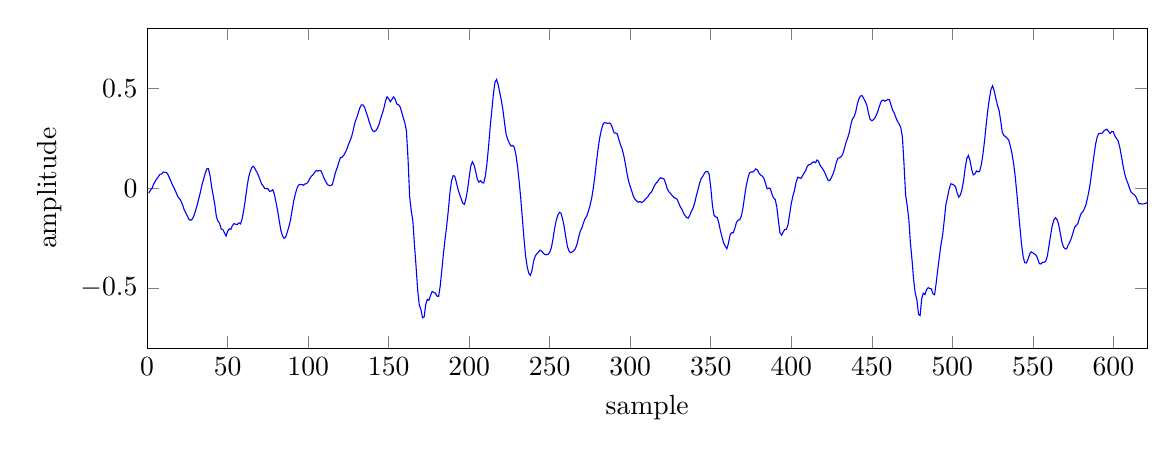
\begin{tikzpicture}

\begin{axis}[%
width=5in,
height=1.6in,
at={(0.756437in,0.480047in)},
scale only axis,
xmin=0,
xmax=621,
xlabel={sample},
ymin=-0.8,
ymax=0.8,
ylabel={amplitude}
]
\addplot [color=blue,solid,forget plot]
  table[row sep=crcr]{%
1	-0.0246930662542582\\
2	-0.0109512591734529\\
3	-0.00150964595377445\\
4	0.0200851950794458\\
5	0.0346970446407795\\
6	0.0469654463231564\\
7	0.0584426075220108\\
8	0.0699233785271645\\
9	0.0708834603428841\\
10	0.081192709505558\\
11	0.0796012058854103\\
12	0.0789244025945663\\
13	0.0667674988508224\\
14	0.0480437465012074\\
15	0.0297445803880692\\
16	0.0120505569502711\\
17	-0.00418582512065768\\
18	-0.0218950361013412\\
19	-0.0417479388415813\\
20	-0.0514114275574684\\
21	-0.0636742934584618\\
22	-0.0839403122663498\\
23	-0.107758477330208\\
24	-0.124450176954269\\
25	-0.139232888817787\\
26	-0.1562559902668\\
27	-0.160254970192909\\
28	-0.154343396425247\\
29	-0.139072716236115\\
30	-0.113095566630363\\
31	-0.0862964391708374\\
32	-0.0538809522986412\\
33	-0.0215533468872309\\
34	0.0159980319440365\\
35	0.0438490062952042\\
36	0.0727146565914154\\
37	0.0966997593641281\\
38	0.0982832089066505\\
39	0.0651051476597786\\
40	0.00904000457376242\\
41	-0.0364017225801945\\
42	-0.0819018483161926\\
43	-0.143239185214043\\
44	-0.16458922624588\\
45	-0.175221368670464\\
46	-0.204255178570747\\
47	-0.206088989973068\\
48	-0.222350463271141\\
49	-0.239400565624237\\
50	-0.214422702789307\\
51	-0.203057155013084\\
52	-0.20536670088768\\
53	-0.185857012867928\\
54	-0.176879540085793\\
55	-0.180236294865608\\
56	-0.181642577052116\\
57	-0.173125743865967\\
58	-0.178467601537704\\
59	-0.152585595846176\\
60	-0.108231291174889\\
61	-0.0557241998612881\\
62	0.00428745616227388\\
63	0.054716806858778\\
64	0.0835389047861099\\
65	0.103966973721981\\
66	0.109565086662769\\
67	0.0976467803120613\\
68	0.0820968449115753\\
69	0.0655762776732445\\
70	0.0444222129881382\\
71	0.022629277780652\\
72	0.0122606558725238\\
73	-0.00154816871508956\\
74	-0.00222908123396337\\
75	-0.0029375683516264\\
76	-0.0156994387507439\\
77	-0.0139352474361658\\
78	-0.00759603781625628\\
79	-0.030378445982933\\
80	-0.0703174620866776\\
81	-0.11095804721117\\
82	-0.161151081323624\\
83	-0.209878981113434\\
84	-0.23674938082695\\
85	-0.250156044960022\\
86	-0.244728595018387\\
87	-0.219889238476753\\
88	-0.193096116185188\\
89	-0.159646511077881\\
90	-0.111086189746857\\
91	-0.0641426369547844\\
92	-0.0294709261506796\\
93	-0.000999521464109421\\
94	0.0155365597456694\\
95	0.018827386200428\\
96	0.0185498520731926\\
97	0.0150090223178267\\
98	0.0212981216609478\\
99	0.0229816082865\\
100	0.0325818173587322\\
101	0.0480249188840389\\
102	0.0599651373922825\\
103	0.0671136751770973\\
104	0.079506941139698\\
105	0.0883503258228302\\
106	0.0854562446475029\\
107	0.0884069502353668\\
108	0.0868376493453979\\
109	0.0675879418849945\\
110	0.0468888767063618\\
111	0.0320933349430561\\
112	0.0178559832274914\\
113	0.0139573235064745\\
114	0.0126845557242632\\
115	0.0180925335735083\\
116	0.0492000766098499\\
117	0.0809527561068535\\
118	0.101717479526997\\
119	0.128954067826271\\
120	0.152744978666306\\
121	0.154858931899071\\
122	0.163890987634659\\
123	0.178015649318695\\
124	0.194610133767128\\
125	0.218136876821518\\
126	0.237434089183807\\
127	0.258943557739258\\
128	0.291455507278442\\
129	0.327491670846939\\
130	0.34998893737793\\
131	0.373387813568115\\
132	0.400433033704758\\
133	0.416377872228622\\
134	0.416516602039337\\
135	0.40499609708786\\
136	0.380071043968201\\
137	0.356820702552795\\
138	0.329572975635529\\
139	0.304919958114624\\
140	0.287622392177582\\
141	0.282936632633209\\
142	0.288275361061096\\
143	0.299829572439194\\
144	0.319395214319229\\
145	0.348428189754486\\
146	0.372637242078781\\
147	0.399528861045837\\
148	0.436088383197784\\
149	0.457315891981125\\
150	0.446670055389404\\
151	0.43244731426239\\
152	0.443736702203751\\
153	0.456703960895538\\
154	0.445595145225525\\
155	0.421007573604584\\
156	0.418013989925385\\
157	0.408350259065628\\
158	0.382829427719116\\
159	0.353656977415085\\
160	0.327848017215729\\
161	0.286901742219925\\
162	0.14727421104908\\
163	-0.0404925495386124\\
164	-0.113836526870728\\
165	-0.163777410984039\\
166	-0.284175395965576\\
167	-0.392490237951279\\
168	-0.510205447673798\\
169	-0.584366261959076\\
170	-0.60602593421936\\
171	-0.648131608963013\\
172	-0.643293082714081\\
173	-0.581106543540955\\
174	-0.555464327335358\\
175	-0.560631811618805\\
176	-0.536024570465088\\
177	-0.515920758247375\\
178	-0.521686255931854\\
179	-0.524960279464722\\
180	-0.539381325244904\\
181	-0.541047096252441\\
182	-0.488138854503632\\
183	-0.408703565597534\\
184	-0.326303631067276\\
185	-0.254035532474518\\
186	-0.188940867781639\\
187	-0.112615369260311\\
188	-0.0238988734781742\\
189	0.0359717793762684\\
190	0.0624470114707947\\
191	0.0605616569519043\\
192	0.0297376923263073\\
193	-0.00429357914254069\\
194	-0.0296843778342009\\
195	-0.0518635250627995\\
196	-0.0754081904888153\\
197	-0.0805699899792671\\
198	-0.051627941429615\\
199	-0.00592223647981882\\
200	0.0571507662534714\\
201	0.112649820744991\\
202	0.132520362734795\\
203	0.116789296269417\\
204	0.0837085619568825\\
205	0.0456103719770908\\
206	0.0305787809193134\\
207	0.0375507809221745\\
208	0.0280714835971594\\
209	0.0260411445051432\\
210	0.0605162568390369\\
211	0.122159361839294\\
212	0.208015382289886\\
213	0.30428484082222\\
214	0.386517584323883\\
215	0.469670563936234\\
216	0.530331492424011\\
217	0.543778002262115\\
218	0.517246007919312\\
219	0.47705015540123\\
220	0.437001585960388\\
221	0.387675195932388\\
222	0.322800934314728\\
223	0.265819996595383\\
224	0.242622524499893\\
225	0.223840072751045\\
226	0.210936740040779\\
227	0.213792368769646\\
228	0.205541521310806\\
229	0.166745901107788\\
230	0.110366344451904\\
231	0.0349541343748569\\
232	-0.0506618060171604\\
233	-0.1499253064394\\
234	-0.251119673252106\\
235	-0.338095158338547\\
236	-0.392690598964691\\
237	-0.426016747951508\\
238	-0.435901194810867\\
239	-0.409926116466522\\
240	-0.364676415920258\\
241	-0.338947653770447\\
242	-0.327855497598648\\
243	-0.319006949663162\\
244	-0.309591263532639\\
245	-0.315148115158081\\
246	-0.324657529592514\\
247	-0.331977635622025\\
248	-0.332711100578308\\
249	-0.33024275302887\\
250	-0.320050776004791\\
251	-0.298074007034302\\
252	-0.254788815975189\\
253	-0.202584818005562\\
254	-0.16231082379818\\
255	-0.134733110666275\\
256	-0.120831966400146\\
257	-0.125127762556076\\
258	-0.154399484395981\\
259	-0.193353086709976\\
260	-0.2449761480093\\
261	-0.292626351118088\\
262	-0.314509838819504\\
263	-0.322929263114929\\
264	-0.318441033363342\\
265	-0.311486393213272\\
266	-0.301177054643631\\
267	-0.277869194746017\\
268	-0.243947833776474\\
269	-0.213395446538925\\
270	-0.197965785861015\\
271	-0.171929270029068\\
272	-0.151400655508041\\
273	-0.139400884509087\\
274	-0.114746458828449\\
275	-0.0867714956402779\\
276	-0.0516235008835793\\
277	-0.00264675612561405\\
278	0.0575350448489189\\
279	0.13057042658329\\
280	0.195923119783401\\
281	0.250391006469727\\
282	0.289175927639008\\
283	0.319113492965698\\
284	0.327995389699936\\
285	0.326261103153229\\
286	0.324167788028717\\
287	0.326539367437363\\
288	0.320190966129303\\
289	0.299414128065109\\
290	0.276934057474136\\
291	0.275761902332306\\
292	0.270932048559189\\
293	0.24077320098877\\
294	0.216350972652435\\
295	0.194614320993423\\
296	0.161978140473366\\
297	0.120786547660828\\
298	0.0732406228780746\\
299	0.0343876332044601\\
300	0.00798436440527439\\
301	-0.0162484310567379\\
302	-0.0416704230010509\\
303	-0.055554062128067\\
304	-0.0636329427361488\\
305	-0.0704906061291695\\
306	-0.0666074231266975\\
307	-0.0716690272092819\\
308	-0.0677271857857704\\
309	-0.0584194548428059\\
310	-0.0502765960991383\\
311	-0.0422277823090553\\
312	-0.0274339187890291\\
313	-0.0205110404640436\\
314	-0.00592227978631854\\
315	0.0124256331473589\\
316	0.0249801315367222\\
317	0.0329934097826481\\
318	0.0469017848372459\\
319	0.0523563101887703\\
320	0.0487438589334488\\
321	0.045920941978693\\
322	0.0238619334995747\\
323	-0.00302410311996937\\
324	-0.0175543799996376\\
325	-0.0264733415096998\\
326	-0.0360381193459034\\
327	-0.0452403277158737\\
328	-0.0499574653804302\\
329	-0.0542202480137348\\
330	-0.0717371702194214\\
331	-0.0920393094420433\\
332	-0.104536794126034\\
333	-0.122203774750233\\
334	-0.136648803949356\\
335	-0.146831393241882\\
336	-0.14957694709301\\
337	-0.134781628847122\\
338	-0.114222869277\\
339	-0.099804162979126\\
340	-0.0740013718605042\\
341	-0.0392816811800003\\
342	-0.00962181761860847\\
343	0.0227288864552975\\
344	0.0478480011224747\\
345	0.0584394782781601\\
346	0.0741886273026466\\
347	0.0828270390629768\\
348	0.0842625722289085\\
349	0.0699168294668198\\
350	0.00411017425358295\\
351	-0.0834241062402725\\
352	-0.135274335741997\\
353	-0.143291369080544\\
354	-0.146022811532021\\
355	-0.173438772559166\\
356	-0.212720051407814\\
357	-0.244060412049294\\
358	-0.273779004812241\\
359	-0.289729952812195\\
360	-0.302414804697037\\
361	-0.274505823850632\\
362	-0.233290761709213\\
363	-0.222416907548904\\
364	-0.22253081202507\\
365	-0.199262425303459\\
366	-0.169337317347527\\
367	-0.159613817930222\\
368	-0.157760426402092\\
369	-0.139391779899597\\
370	-0.0991045758128166\\
371	-0.0412341505289078\\
372	0.0111712822690606\\
373	0.0483754985034466\\
374	0.0760266333818436\\
375	0.0810916274785995\\
376	0.0805717408657074\\
377	0.0881712734699249\\
378	0.096536785364151\\
379	0.0913260206580162\\
380	0.074830062687397\\
381	0.0654525756835938\\
382	0.0606594420969486\\
383	0.0497056990861893\\
384	0.0236151274293661\\
385	-0.00299435690976679\\
386	0.00140368903521448\\
387	-0.0023518935777247\\
388	-0.0291524101048708\\
389	-0.0490568168461323\\
390	-0.0557457953691483\\
391	-0.0932002365589142\\
392	-0.162884697318077\\
393	-0.223134413361549\\
394	-0.23442168533802\\
395	-0.218448132276535\\
396	-0.206071525812149\\
397	-0.205656111240387\\
398	-0.181155830621719\\
399	-0.128510043025017\\
400	-0.0762601718306541\\
401	-0.0394606292247772\\
402	-0.00937995128333569\\
403	0.0298291314393282\\
404	0.0550615414977074\\
405	0.0523985102772713\\
406	0.0491326153278351\\
407	0.0623609274625778\\
408	0.0759602040052414\\
409	0.089863583445549\\
410	0.11069293320179\\
411	0.117786437273026\\
412	0.11895989626646\\
413	0.128384798765182\\
414	0.132012590765953\\
415	0.127426579594612\\
416	0.141273409128189\\
417	0.132910579442978\\
418	0.112596765160561\\
419	0.102521531283855\\
420	0.0902106463909149\\
421	0.0738431885838509\\
422	0.054602362215519\\
423	0.0388106815516949\\
424	0.0394822135567665\\
425	0.0546577423810959\\
426	0.0723937749862671\\
427	0.0966623425483704\\
428	0.130758970975876\\
429	0.150017008185387\\
430	0.152579009532928\\
431	0.157857984304428\\
432	0.171196609735489\\
433	0.200112476944923\\
434	0.228981852531433\\
435	0.250662297010422\\
436	0.277911484241486\\
437	0.31851053237915\\
438	0.346849292516708\\
439	0.357346415519714\\
440	0.380888789892197\\
441	0.420735359191895\\
442	0.447029262781143\\
443	0.461872100830078\\
444	0.462273925542831\\
445	0.448150455951691\\
446	0.433449804782867\\
447	0.412003874778748\\
448	0.373867899179459\\
449	0.343589842319489\\
450	0.338014841079712\\
451	0.342062890529633\\
452	0.352864801883698\\
453	0.368585139513016\\
454	0.390867054462433\\
455	0.4163778424263\\
456	0.43626144528389\\
457	0.440757185220718\\
458	0.435244292020798\\
459	0.43885725736618\\
460	0.443904608488083\\
461	0.441663503646851\\
462	0.414435803890228\\
463	0.389604389667511\\
464	0.375652194023132\\
465	0.35191148519516\\
466	0.334744602441788\\
467	0.320273458957672\\
468	0.303240716457367\\
469	0.257086575031281\\
470	0.120977774262428\\
471	-0.0339391268789768\\
472	-0.0882608219981194\\
473	-0.157026648521423\\
474	-0.275673180818558\\
475	-0.360380113124847\\
476	-0.459677517414093\\
477	-0.525279998779297\\
478	-0.558098077774048\\
479	-0.629707276821136\\
480	-0.636797189712524\\
481	-0.551932990550995\\
482	-0.524585485458374\\
483	-0.531986653804779\\
484	-0.507475137710571\\
485	-0.497414112091064\\
486	-0.5013747215271\\
487	-0.503416895866394\\
488	-0.527956187725067\\
489	-0.532597780227661\\
490	-0.473168849945068\\
491	-0.404149502515793\\
492	-0.341049313545227\\
493	-0.280269712209702\\
494	-0.232950612902641\\
495	-0.159658163785934\\
496	-0.0828282311558723\\
497	-0.0448275730013847\\
498	-0.00613126810640097\\
499	0.0218491293489933\\
500	0.019827775657177\\
501	0.0156100913882256\\
502	0.00721522141247988\\
503	-0.0231753215193748\\
504	-0.0446735844016075\\
505	-0.0335372537374496\\
506	-0.00624906644225121\\
507	0.0381038077175617\\
508	0.10125645250082\\
509	0.149203911423683\\
510	0.163538590073586\\
511	0.138059809803963\\
512	0.0950194001197815\\
513	0.0666819140315056\\
514	0.071422703564167\\
515	0.086234875023365\\
516	0.0814853459596634\\
517	0.0852532461285591\\
518	0.117530554533005\\
519	0.169255539774895\\
520	0.235485553741455\\
521	0.316461741924286\\
522	0.388104289770126\\
523	0.446198672056198\\
524	0.494040846824646\\
525	0.51188850402832\\
526	0.488356500864029\\
527	0.450187832117081\\
528	0.416626036167145\\
529	0.390448421239853\\
530	0.339474081993103\\
531	0.281103998422623\\
532	0.262895315885544\\
533	0.258867919445038\\
534	0.25046318769455\\
535	0.241421803832054\\
536	0.212482988834381\\
537	0.175100445747375\\
538	0.12782384455204\\
539	0.0632240027189255\\
540	-0.0196083765476942\\
541	-0.107695326209068\\
542	-0.195933938026428\\
543	-0.281486064195633\\
544	-0.343332707881927\\
545	-0.372591227293015\\
546	-0.37395179271698\\
547	-0.354530990123749\\
548	-0.329846262931824\\
549	-0.317908138036728\\
550	-0.322896420955658\\
551	-0.329117894172668\\
552	-0.334650188684464\\
553	-0.352013826370239\\
554	-0.376838117837906\\
555	-0.378807097673416\\
556	-0.371410101652145\\
557	-0.370089828968048\\
558	-0.365597069263458\\
559	-0.340193808078766\\
560	-0.289849191904068\\
561	-0.23712058365345\\
562	-0.189335823059082\\
563	-0.160537421703339\\
564	-0.147431284189224\\
565	-0.156488940119743\\
566	-0.179591715335846\\
567	-0.222201064229012\\
568	-0.267128556966782\\
569	-0.293218463659286\\
570	-0.302759438753128\\
571	-0.30243769288063\\
572	-0.283375382423401\\
573	-0.26865229010582\\
574	-0.248775362968445\\
575	-0.221823841333389\\
576	-0.194331884384155\\
577	-0.185959577560425\\
578	-0.17555958032608\\
579	-0.149058103561401\\
580	-0.126138538122177\\
581	-0.118643909692764\\
582	-0.102947920560837\\
583	-0.0829823538661003\\
584	-0.0473890043795109\\
585	-0.00764255365356803\\
586	0.0438558608293533\\
587	0.107991732656956\\
588	0.164382293820381\\
589	0.221208482980728\\
590	0.256764054298401\\
591	0.274437069892883\\
592	0.274166971445084\\
593	0.274269431829453\\
594	0.285065412521362\\
595	0.291507214307785\\
596	0.29481452703476\\
597	0.284308612346649\\
598	0.274060159921646\\
599	0.283846706151962\\
600	0.282563030719757\\
601	0.260126322507858\\
602	0.248791575431824\\
603	0.236106485128403\\
604	0.204707190394402\\
605	0.160638108849525\\
606	0.114030033349991\\
607	0.0734585970640182\\
608	0.0454584769904613\\
609	0.0259404927492142\\
610	0.00068305351305753\\
611	-0.0187134835869074\\
612	-0.0270869210362434\\
613	-0.0328924506902695\\
614	-0.042515579611063\\
615	-0.0616966150701046\\
616	-0.078101709485054\\
617	-0.0774170756340027\\
618	-0.0787554085254669\\
619	-0.0781508013606071\\
620	-0.0761454403400421\\
621	-0.0699243322014809\\
};
\end{axis}
\end{tikzpicture}%

\caption{input signal around an analysis time instant}
\label{fig:s}
\end{figure}

The next step is to generate $\matr{R}$ by resampling the DTFT of a squared analysis window. We first show the DTFT of a squared hamming window before resampling in figure \ref{fig:sqhamm}.

\begin{figure}[H]
\centering
% This file was created by matlab2tikz.
% Minimal pgfplots version: 1.3
%
%The latest updates can be retrieved from
%  http://www.mathworks.com/matlabcentral/fileexchange/22022-matlab2tikz
%where you can also make suggestions and rate matlab2tikz.
%
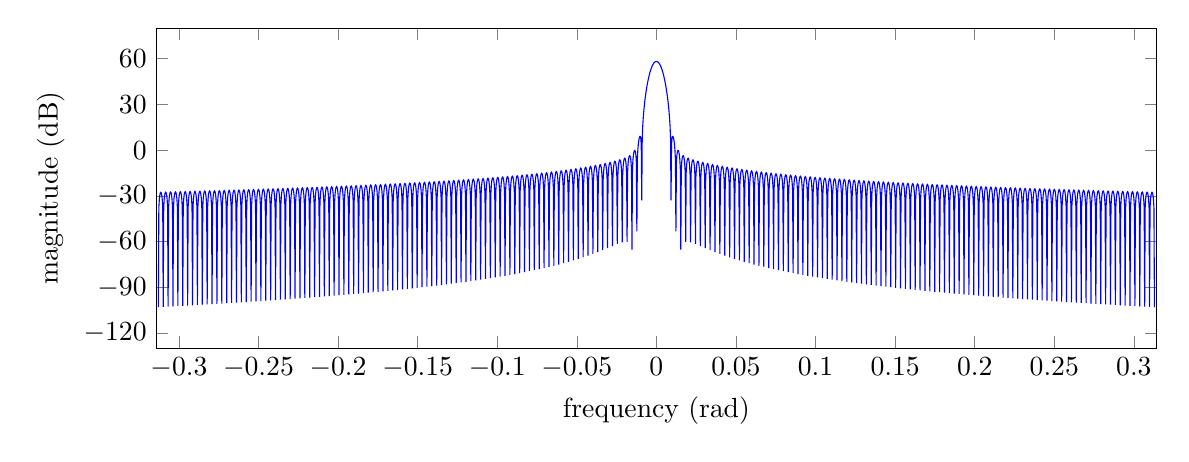
\begin{tikzpicture}

\begin{axis}[
width=5in,
height=1.6in,
at={(1.091431in,0.417184in)},
scale only axis,
unbounded coords=jump,
xmin=-0.314159265358979,
xmax=0.314159265358979,
xlabel={frequency (rad)},
ymin=-130,
ymax=80,
ytick={-120,  -90,  -60,  -30,    0,   30,   60},
xticklabel style={/pgf/number format/fixed},
ylabel={magnitude (dB)}
]
\addplot [color=blue,solid,forget plot]
  table[row sep=crcr]{%
-0.312932080728671	-103.047383503594\\
-0.312625284571094	-37.9352917684934\\
-0.312318488413517	-32.3395880713616\\
-0.312011692255939	-29.5553910357496\\
-0.311704896098362	-28.141360829615\\
-0.311398099940785	-27.6965360785851\\
-0.311091303783208	-28.1234489158977\\
-0.310784507625631	-29.5193373459398\\
-0.310477711468054	-32.2846487973438\\
-0.310170915310477	-37.8583162790573\\
-0.3098641191529	-102.875796315252\\
-0.309557322995322	-37.8505610133483\\
-0.309250526837745	-32.2547471081055\\
-0.308943730680168	-29.4704554673575\\
-0.308636934522591	-28.0563342043086\\
-0.308330138365014	-27.6114193685022\\
-0.308023342207437	-28.0382419359481\\
-0.30771654604986	-29.4340387452984\\
-0.307409749892282	-32.1992546081336\\
-0.307102953734705	-37.7728102712921\\
-0.306796157577128	-102.702521524044\\
-0.306489361419551	-37.7649768938795\\
-0.306182565261974	-32.1690506037075\\
-0.305875769104397	-29.3846624885065\\
-0.30556897294682	-27.9704483677664\\
-0.305262176789243	-27.5254416638538\\
-0.304955380631665	-27.9521721725678\\
-0.304648584474088	-29.3478755434837\\
-0.304341788316511	-32.1129939188757\\
-0.304034992158934	-37.6864355382112\\
-0.303728196001357	-102.527525224479\\
-0.30342139984378	-37.6785225050626\\
-0.303114603686203	-32.0824815875891\\
-0.302807807528626	-29.2979950723216\\
-0.302501011371048	-27.883686238838\\
-0.302194215213471	-27.4385858296878\\
-0.301887419055894	-27.8652224367409\\
-0.301580622898317	-29.2608304965579\\
-0.30127382674074	-32.0258494281407\\
-0.300967030583163	-37.5991747108765\\
-0.300660234425586	-102.350772477225\\
-0.300353438268009	-37.5911804315663\\
-0.300046642110431	-31.9950225762161\\
-0.299739845952854	-29.2104356766941\\
-0.299433049795277	-27.7960302189402\\
-0.2991262536377	-27.3508342114388\\
-0.298819457480123	-27.7773750176963\\
-0.298512661322546	-29.1728858365449\\
-0.298205865164969	-31.9378033081764\\
-0.297899069007391	-37.5110098912166\\
-0.297592272849814	-102.172227284236\\
-0.297285476692237	-37.5029327270628\\
-0.29697868053466	-31.9066555522691\\
-0.296671884377083	-29.1219662233341\\
-0.296365088219506	-27.7074621710004\\
-0.296058292061929	-27.2621686137594\\
-0.295751495904352	-27.6886116615639\\
-0.295444699746774	-29.0840232500632\\
-0.295137903589197	-31.8488371831254\\
-0.29483110743162	-37.4219226303782\\
-0.294524311274043	-101.991852533655\\
-0.294217515116466	-37.413760892477\\
-0.293910718958889	-31.8173619427476\\
-0.293603922801312	-29.0325680757559\\
-0.293297126643735	-27.6179633973195\\
-0.292990330486157	-27.1725702782651\\
-0.29268353432858	-27.5989135490136\\
-0.292376738171003	-28.9942238556907\\
-0.292069942013426	-31.7589321069336\\
-0.291763145855849	-37.3318939059468\\
-0.291456349698272	-101.809609956508\\
-0.291149553540695	-37.3236458532302\\
-0.290842757383118	-31.7271225959476\\
-0.29053596122554	-28.9422220161178\\
-0.290229165067963	-27.5275146162877\\
-0.289922368910386	-27.0820198601256\\
-0.289615572752809	-27.508261271719\\
-0.289308776595232	-28.90346818058\\
-0.289001980437655	-31.6680685390211\\
-0.288695184280078	-37.2409040979893\\
-0.288388388122501	-101.625459872335\\
-0.288081591964923	-37.2325679345829\\
-0.287774795807346	-31.6359177572291\\
-0.287467999649769	-28.8509082208575\\
-0.287161203492192	-27.436095937884\\
-0.286854407334615	-26.9904974034293\\
-0.286547611177038	-27.416634807589\\
-0.286240815019461	-28.8117361352732\\
-0.285934018861884	-31.5762263194963\\
-0.285627222704306	-37.1489329637164\\
-0.285320426546729	-101.439362169963\\
-0.285013630389152	-37.1405068374891\\
-0.284706834231575	-31.543727043514\\
-0.284400038073998	-28.7586062350375\\
-0.284093241916421	-27.3436868378796\\
-0.283786445758844	-26.8979823152454\\
-0.283479649601266	-27.3240134946865\\
-0.283172853443689	-28.7190069876132\\
-0.282866057286112	-31.4833846427236\\
-0.282559261128535	-37.0559596115123\\
-0.282252464970958	-101.251274184656\\
-0.281945668813381	-37.0474416107254\\
-0.281638872655804	-31.4505294164202\\
-0.281332076498227	-28.6652949452948\\
-0.281025280340649	-27.2502661306638\\
-0.280718484183072	-26.8044533382986\\
-0.280411688025495	-27.2303760037501\\
-0.280104891867918	-28.6252593350847\\
-0.279798095710341	-31.3895220295267\\
-0.279491299552764	-36.9619624717617\\
-0.279184503395187	-101.061152715707\\
-0.27887770723761	-36.9533506233717\\
-0.278570911080032	-31.3563031538975\\
-0.278264114922455	-28.5709525515036\\
-0.277957318764878	-27.1558119406025\\
-0.277650522607301	-26.7098885221663\\
-0.277343726449724	-27.1357003092308\\
-0.277036930292147	-28.5304710756829\\
-0.27673013413457	-31.2946162978845\\
-0.276423337976993	-36.8669192685294\\
-0.276116541819415	-100.868952926781\\
-0.275809745661838	-36.858211534928\\
-0.275502949504261	-31.2610258206426\\
-0.275196153346684	-28.475556536462\\
-0.274889357189107	-27.0603016718349\\
-0.27458256103153	-26.6142651929041\\
-0.274275764873953	-27.0399636587306\\
-0.273968968716375	-28.43461937719\\
-0.273662172558798	-31.198644532025\\
-0.273355376401221	-36.7708069878378\\
-0.273048580243644	-100.674628688609\\
-0.272741784086067	-36.762001264639\\
-0.27243498792849	-31.1646742360701\\
-0.272128191770913	-28.3790836344875\\
-0.271821395613336	-26.9637119764031\\
-0.271514599455759	-26.5175599209932\\
-0.271207803298181	-26.9431425408289\\
-0.270901007140604	-28.3376806447508\\
-0.270594210983027	-31.1015830498009\\
-0.27028741482545	-36.6736018449303\\
-0.269980618667873	-100.478131528247\\
-0.269673822510296	-36.6646959572941\\
-0.269367026352719	-31.0672244415997\\
-0.269060230195141	-28.2815097978277\\
-0.268753434037564	-26.8660187206197\\
-0.268446637879987	-26.4197484874977\\
-0.26813984172241	-26.8452126509194\\
-0.267833045564833	-28.2396304866338\\
-0.267526249407256	-31.0034073682411\\
-0.267219453249679	-36.5752792495745\\
-0.266912657092102	-100.27941252185\\
-0.266605860934524	-36.5662709495526\\
-0.266299064776947	-30.9686516652734\\
-0.26599226861937	-28.1828101613826\\
-0.265685472461793	-26.7671969494605\\
-0.265378676304216	-26.320805848315\\
-0.265071880146639	-26.7461488553732\\
-0.264765083989062	-28.1404436780561\\
-0.264458287831485	-30.9040921672026\\
-0.264151491673907	-36.4758137693893\\
-0.26384469551633	-100.078420262085\\
-0.263537899358753	-36.4667007325096\\
-0.263231103201176	-30.8689302847503\\
-0.262924307043599	-28.0829590052197\\
-0.262617510886022	-26.6672208491232\\
-0.262310714728445	-26.2207060963827\\
-0.262003918570868	-26.6459251534607\\
-0.26169712241329	-28.0400941229651\\
-0.261390326255713	-30.8036112506193\\
-0.261083530098136	-36.375179091084\\
-0.260776733940559	-99.8751017559717\\
-0.260469937782982	-36.3659589128565\\
-0.260163141625405	-30.7680337877934\\
-0.259856345467828	-27.9819297153602\\
-0.25954954931025	-26.5660637071649\\
-0.259242753152673	-26.1194224217066\\
-0.258935956995096	-26.5445146371633\\
-0.258629160837519	-27.9385548134411\\
-0.258322364679942	-30.7019375063178\\
-0.258015568522365	-36.2733479794329\\
-0.257708772364788	-99.6694021467792\\
-0.257401976207211	-36.2640181716614\\
-0.257095180049633	-30.6659347312745\\
-0.256788383892056	-27.8796947417034\\
-0.256481587734479	-26.4636978705156\\
-0.256174791576902	-26.0169270690535\\
-0.255867995419325	-26.4418894485489\\
-0.255561199261748	-27.835797787152\\
-0.255254403104171	-30.5990428623865\\
-0.254947606946594	-36.1702922338556\\
-0.254640810789016	-99.4612644541161\\
-0.254334014631439	-36.1608502207339\\
-0.254027218473862	-30.5626046966666\\
-0.253720422316285	-27.776225553911\\
-0.253413626158708	-26.3600947009211\\
-0.253106830001131	-25.9131912931483\\
-0.252800033843554	-26.3380207348152\\
-0.252493237685977	-27.7317940817137\\
-0.252186441528399	-30.4948982417851\\
-0.251879645370822	-36.0659826422993\\
-0.251572849213245	-99.2506303411461\\
-0.251266053055668	-36.0564257563833\\
-0.250959256898091	-30.458014243725\\
-0.250652460740514	-27.6714925944903\\
-0.250345664582937	-26.255224527808\\
-0.250038868425359	-25.8081853111915\\
-0.249732072267782	-26.2328786003916\\
-0.249425276110205	-27.6265136867526\\
-0.249118479952628	-30.3894735138818\\
-0.248811683795051	-35.9603889329445\\
-0.248504887637474	-99.0374382893941\\
-0.248198091479897	-35.9507144104138\\
-0.24789129532232	-30.352132861022\\
-0.247584499164742	-27.5654652290381\\
-0.247277703007165	-26.1490565981682\\
-0.246970906849588	-25.7018782525095\\
-0.246664110692011	-26.1264320563325\\
-0.246357314534434	-27.5199254928854\\
-0.246050518376857	-30.2827374432024\\
-0.24574372221928	-35.8534797215863\\
-0.245436926061703	-98.8216252242765\\
-0.245130129904125	-35.8436846981261\\
-0.244823333746548	-30.2449289136224\\
-0.244516537588971	-27.4581116935833\\
-0.244209741431394	-26.0415590234997\\
-0.243902945273817	-25.5942381051234\\
-0.24359614911624	-26.0186489665353\\
-0.243289352958663	-27.4119972376092\\
-0.242982556801086	-30.1746576347902\\
-0.242675760643508	-35.7452224575766\\
-0.242368964485931	-98.6031255356684\\
-0.242062168328354	-35.7353039631251\\
-0.241755372170777	-30.1363695873008\\
-0.2414485760132	-27.349399038436\\
-0.241141779855623	-25.9326987234569\\
-0.240834983698046	-25.4852316590109\\
-0.240528187540469	-25.9094959906354\\
-0.240221391382891	-27.3026954478103\\
-0.239914595225314	-30.0652004764963\\
-0.239607799067737	-35.6355833650725\\
-0.23930100291016	-98.3818711343146\\
-0.238994206752583	-35.6255383186863\\
-0.238687410595006	-30.0264208295698\\
-0.238380614437429	-27.2392930687853\\
-0.238073818279851	-25.8224413659149\\
-0.237767022122274	-25.3748244458112\\
-0.237460225964697	-25.7989385233219\\
-0.23715342980712	-27.1919853786914\\
-0.236846633649543	-29.9543310773898\\
-0.236539837491966	-35.5245273811092\\
-0.236233041334389	-98.1577913222717\\
-0.235926245176812	-35.5143525854234\\
-0.235619449019234	-29.9150472867826\\
-0.235312652861657	-27.1277582813753\\
-0.23500585670408	-25.710751303278\\
-0.234699060546503	-25.2629806747067\\
-0.234392264388926	-25.6869406297929\\
-0.234085468231349	-27.0798309487908\\
-0.233778672073772	-29.8420132023473\\
-0.233471875916195	-35.4120180896328\\
-0.233165079758617	-97.9308126608418\\
-0.23285828360104	-35.4017102249723\\
-0.232551487443463	-29.8022122372756\\
-0.232244691285886	-27.0147577971802\\
-0.231937895128309	-25.5975915046935\\
-0.231631098970732	-25.1496631641845\\
-0.231324302813155	-25.5734649770645\\
-0.231017506655578	-26.9661946708246\\
-0.230710710498	-29.7282092024033\\
-0.230403914340423	-35.2980176512731\\
-0.230097118182846	-97.7008588295979\\
-0.229790322025269	-35.2875732693934\\
-0.229483525867692	-29.6878775201782\\
-0.229176729710115	-26.9002532897057\\
-0.228869933552538	-25.4829234838628\\
-0.228563137394961	-25.0348332693603\\
-0.228256341237383	-25.458472760802\\
-0.227949545079806	-26.8510375780177\\
-0.227642748922229	-29.612879940555\\
-0.227335952764652	-35.1824867285224\\
-0.227029156607075	-97.4678504706146\\
-0.226722360449498	-35.1719022459439\\
-0.226415564291921	-29.5720034595488\\
-0.226108768134344	-26.7842049085775\\
-0.225801971976766	-25.3667072221008\\
-0.225495175819189	-24.9184508045131\\
-0.225188379661612	-25.3419236273251\\
-0.224881583504035	-26.7343191455676\\
-0.224574787346458	-29.4959847126539\\
-0.224267991188881	-35.0653844059494\\
-0.223961195031304	-97.2317050279091\\
-0.223654398873727	-35.0546560968663\\
-0.223347602716149	-29.4545487834701\\
-0.223040806558572	-26.6665711980458\\
-0.222734010400995	-25.2489010862707\\
-0.222427214243418	-24.8004739604502\\
-0.222120418085841	-25.223775590401\\
-0.221813621928264	-26.6159972068513\\
-0.221506825770687	-29.3774811629987\\
-0.221200029613109	-34.9466681050628\\
-0.220893233455532	-96.9923365696316\\
-0.220586437297955	-34.9357920937788\\
-0.220279641140378	-29.3354705376965\\
-0.219972844982801	-26.5473090099941\\
-0.219666048825224	-25.1294617411746\\
-0.219359252667647	-24.6808592162856\\
-0.21905245651007	-25.1039849424021\\
-0.218745660352492	-26.4960278639512\\
-0.218438864194915	-29.2573251941948\\
-0.218132068037338	-34.8262934933743\\
-0.217825271879761	-96.7496556096788\\
-0.217518475722184	-34.815265746241\\
-0.217211679564607	-29.2147239934127\\
-0.21690488340703	-26.4263734110057\\
-0.216598087249453	-25.0083440559524\\
-0.216291291091875	-24.5595612451731\\
-0.215984494934298	-24.9825061593701\\
-0.215677698776721	-26.3743653920326\\
-0.215370902619144	-29.1354708708087\\
-0.215064106461567	-34.7042143872055\\
-0.21475731030399	-96.5035689010643\\
-0.214450514146413	-34.6930307040109\\
-0.214143717988835	-29.0922625486141\\
-0.213836921831258	-26.3037175829964\\
-0.213530125673681	-24.8855010039895\\
-0.213223329516104	-24.4365328134937\\
-0.212916533358527	-24.8592917994764\\
-0.21260973720095	-26.2509621370629\\
-0.212302941043373	-29.0118703163066\\
-0.211996144885796	-34.580382647687\\
-0.211689348728218	-96.2539792305383\\
-0.211382552570641	-34.5690386524629\\
-0.211075756413064	-28.9680376225786\\
-0.210768960255487	-26.1792927168716\\
-0.21046216409791	-24.76088355579\\
-0.210155367940333	-24.3117246729483\\
-0.209848571782756	-24.7342923943272\\
-0.209541775625179	-26.1257684063089\\
-0.209234979467601	-28.8864736027032\\
-0.208928183310024	-34.4547480694052\\
-0.208621387152447	-96.0007851878976\\
-0.20831459099487	-34.443239200598\\
-0.208007794837293	-28.8419985428404\\
-0.207700998679716	-26.0530478986201\\
-0.207394202522139	-24.6344405642172\\
-0.207087406364562	-24.1850854449499\\
-0.206780610206984	-24.6074563324993\\
-0.206473814049407	-25.9987323509996\\
-0.20616701789183	-28.7592286323005\\
-0.205860221734253	-34.3272582610424\\
-0.205553425576676	-95.7438809190696\\
-0.205246629419099	-34.3155797609916\\
-0.204939833261522	-28.7140924240264\\
-0.204633037103945	-25.92492998719\\
-0.204326240946367	-24.506118641444\\
-0.20401944478879	-24.0565614966513\\
-0.203712648631213	-24.4787297346379\\
-0.203405852473636	-25.8697998404707\\
-0.203099056316059	-28.6300810108328\\
-0.202792260158482	-34.1978585173281\\
-0.202485464000905	-95.4831558708065\\
-0.202178667843328	-34.1860054210052\\
-0.20187187168575	-28.5842640378399\\
-0.201565075528173	-25.7948834834307\\
-0.201258279370596	-24.3758620268862\\
-0.200951483213019	-23.926096807875\\
-0.200644687055442	-24.3480563193748\\
-0.200337890897865	-25.7389143270478\\
-0.200031094740288	-28.4989739112562\\
-0.19972429858271	-34.0664916815286\\
-0.199417502425133	-95.2184945015729\\
-0.199110706267556	-34.0544588044629\\
-0.198803910109979	-28.4524556734153\\
-0.198497113952402	-25.6628503893119\\
-0.198190317794825	-24.2436124453217\\
-0.197883521637248	-23.7936328281404\\
-0.197576725479671	-24.2153772592508\\
-0.197269929322093	-25.6060167008405\\
-0.196963133164516	-28.3658479273517\\
-0.196656337006939	-33.9330979976335\\
-0.196349540849362	-94.949775985323\\
-0.196042744691785	-33.9208799229633\\
-0.195735948534208	-28.3186069871786\\
-0.195429152376631	-25.5287700565403\\
-0.195122356219054	-24.1093089543129\\
-0.194815560061476	-23.6591083228924\\
-0.194508763903899	-24.0806310257422\\
-0.194201967746322	-25.4710451335346\\
-0.193895171588745	-28.2306409162208\\
-0.193588375431168	-33.7976149513064\\
-0.193281579273591	-94.6768738817331\\
-0.192974783116014	-33.7852060158701\\
-0.192667986958437	-28.1826548412543\\
-0.192361190800859	-25.39257902362\\
-0.192054394643282	-23.9728877799551\\
-0.191747598485705	-23.5224592079475\\
-0.191440802328128	-23.9437532223913\\
-0.191134006170551	-25.3339349101803\\
-0.190827210012974	-28.0932878286548\\
-0.190520413855397	-33.6599770985575\\
-0.190213617697819	-94.399655786612\\
-0.189906821540242	-33.6473713779499\\
-0.189600025382665	-28.044533129374\\
-0.189293229225088	-25.2542108402742\\
-0.188986433067511	-23.8342821398703\\
-0.188679636909934	-23.3836183710648\\
-0.188372840752357	-23.8046764049402\\
-0.18806604459478	-25.194618247852\\
-0.187759248437202	-27.9537205262396\\
-0.187452452279625	-33.5201158810002\\
-0.187145656122048	-94.11798294924\\
-0.186838859964471	-33.5073071734966\\
-0.186532063806894	-27.9041725891019\\
-0.186225267649317	-25.1135958780556\\
-0.18591847149174	-23.6934220522513\\
-0.185611675334163	-23.2425154794299\\
-0.185304879176585	-23.6633298872398\\
-0.184998083019008	-25.0530240999458\\
-0.184691286861431	-27.8118675839543\\
-0.184384490703854	-33.3779594264156\\
-0.184077694546277	-93.8317098688829\\
-0.1837708983887	-33.3649412356605\\
-0.183464102231123	-27.7615005990899\\
-0.183157306073546	-24.9706611258247\\
-0.182850509915968	-23.5502341296224\\
-0.182543713758391	-23.0990767717055\\
-0.182236917600814	-23.5196395315754\\
-0.181930121443237	-24.9090779447371\\
-0.18162332528566	-27.6676540768606\\
-0.181316529128083	-33.2334323332192\\
-0.181009732970506	-93.5406838449004\\
-0.180702936812929	-33.2201978495653\\
-0.180396140655351	-27.6164409599121\\
-0.180089344497774	-24.8253299686317\\
-0.179782548340197	-23.4046413558388\\
-0.17947575218262	-22.9532248331554\\
-0.179168956025043	-23.3735275218933\\
-0.178862159867466	-24.7627015566654\\
-0.178555363709889	-27.5210013493404\\
-0.178248567552311	-33.0864554372419\\
-0.177941771394734	-93.2447445030742\\
-0.177634975237157	-33.0729975176251\\
-0.17732817907958	-27.4689136568664\\
-0.177021382922003	-24.67752194838\\
-0.176714586764426	-23.2565628446764\\
-0.176407790606849	-22.8048783521715\\
-0.176100994449272	-23.2249121182447\\
-0.175794198291694	-24.6138127586433\\
-0.175487402134117	-27.371826765147\\
-0.17518060597654	-32.936945559091\\
-0.174873809818963	-92.9437232729779\\
-0.174567013661386	-32.9232567052854\\
-0.174260217503809	-27.318834602959\\
-0.173953421346232	-24.5271525044492\\
-0.173646625188655	-23.1059135781775\\
-0.173339829031077	-22.6539518563449\\
-0.1730330328735	-23.0737073905623\\
-0.172726236715923	-24.4623251534817\\
-0.172419440558346	-27.2200434363475\\
-0.172112644400769	-32.7848152301172\\
-0.171805848243192	-92.6374428211406\\
-0.171499052085615	-32.7708875652305\\
-0.171192255928038	-27.1661153600624\\
-0.17088545977046	-24.3741326922512\\
-0.170578663612883	-22.9526041226912\\
-0.170271867455306	-22.5003554260066\\
-0.169965071297729	-22.9198229296697\\
-0.169658275140152	-24.3081478323032\\
-0.169351478982575	-27.0655599289965\\
-0.169044682824998	-32.6299723948035\\
-0.168737886667421	-92.3257164431195\\
-0.168431090509843	-32.6157976378436\\
-0.168124294352266	-27.0106628360051\\
-0.167817498194689	-24.2183688774533\\
-0.167510702037112	-22.7965403203214\\
-0.167203905879535	-22.3439943829059\\
-0.166897109721958	-22.763163533165\\
-0.166590313564381	-24.151185057564\\
-0.166283517406803	-26.9082799431236\\
-0.165976721249226	-32.4723200871305\\
-0.165669925091649	-92.0083473893812\\
-0.165363128934072	-32.457889525441\\
-0.165056332776495	-26.8523789550878\\
-0.164749536618918	-24.0597624033154\\
-0.164442740461341	-22.6376229531951\\
-0.164135944303764	-22.1847689514233\\
-0.163829148146186	-22.603628863543\\
-0.163522351988609	-23.9913359180025\\
-0.163215555831032	-26.7481019643371\\
-0.162908759673455	-32.3117560781512\\
-0.162601963515878	-91.6851281429924\\
-0.162295167358301	-32.2970605375203\\
-0.161988371200724	-26.6911602992042\\
-0.161681575043147	-23.8982092282948\\
-0.161374778885569	-22.4757473776692\\
-0.161067982727992	-22.0225738893874\\
-0.160761186570415	-22.4411130755853\\
-0.160454390412838	-23.828493952519\\
-0.160147594255261	-26.5849188839809\\
-0.159840798097684	-32.1481724916951\\
-0.159534001940107	-91.3558396228818\\
-0.15922720578253	-32.1332023039\\
-0.158920409624952	-26.5268977163951\\
-0.158613613467375	-23.7335995307016\\
-0.158306817309798	-22.3108031252123\\
-0.158000021152221	-21.857298085199\\
-0.157693224994644	-22.275504409686\\
-0.157386428837067	-23.6625467396002\\
-0.15707963267949	-26.4186175844358\\
-0.156772836521913	-31.9814553847079\\
-0.156466040364335	-91.0202503134332\\
-0.156159244206758	-31.9662003522288\\
-0.155852448049181	-26.359475893274\\
-0.155545651891604	-23.5658172767849\\
-0.155238855734027	-22.1426734663023\\
-0.15493205957645	-21.6888241175511\\
-0.154625263418873	-22.1066847473437\\
-0.154318467261295	-23.4933754484755\\
-0.154011671103718	-26.249078485685\\
-0.153704874946141	-31.8114842882966\\
-0.153398078788564	-90.6781153191527\\
-0.153091282630987	-31.7959336459247\\
-0.15278448647341	-26.1887728872853\\
-0.152477690315833	-23.3947397481681\\
-0.152170894158256	-21.971234933195\\
-0.151864098000678	-21.5170277735454\\
-0.151557301843101	-21.9345291245751\\
-0.151250505685524	-23.3208543477022\\
-0.150943709527947	-26.0761750487814\\
-0.15063691337037	-31.6381317050457\\
-0.150330117212793	-90.3291753167991\\
-0.150023321055216	-31.6222740780439\\
-0.149716524897639	-26.0146596142504\\
-0.149409728740061	-23.2202370240105\\
-0.149102932582484	-21.7963567968834\\
-0.148796136424907	-21.3417775204644\\
-0.14848934026733	-21.7589051984372\\
-0.148182544109753	-23.1448502662972\\
-0.147875747952176	-25.8997732312717\\
-0.147568951794599	-31.4612625575575\\
-0.147262155637022	-89.9731554160182\\
-0.146955359479444	-31.4450859160268\\
-0.146648563321867	-25.8369992860364\\
-0.14634176716429	-23.0421714126602\\
-0.146034971006713	-21.6179004929386\\
-0.145728174849136	-21.1629339258152\\
-0.145421378691559	-21.5796726612056\\
-0.145114582533982	-22.9652220018908\\
-0.144807786376405	-25.7197308889619\\
-0.144500990218827	-31.2807335825141\\
-0.14419419406125	-89.6097638983975\\
-0.143887397903673	-31.2642251915627\\
-0.143580601746096	-25.6556467924867\\
-0.143273805588519	-22.8603968268566\\
-0.142967009430942	-21.4357189902037\\
-0.142660213273365	-20.9803490195347\\
-0.142353417115788	-21.396682596011\\
-0.14204662095821	-22.7818196696148\\
-0.141739824800633	-25.5358971176464\\
-0.141433028643056	-31.0963926637681\\
-0.141126232485479	-89.2386908285934\\
-0.140819436327902	-31.0795390290211\\
-0.140512640170325	-25.4704480209649\\
-0.140205844012748	-22.674758095718\\
-0.13989904785517	-21.2496560954856\\
-0.139592251697593	-20.793865591401\\
-0.139285455540016	-21.2097767668797\\
-0.138978659382439	-22.5944839845699\\
-0.138671863224862	-25.3481115275409\\
-0.138365067067285	-30.9080780970549\\
-0.138058270909708	-88.8596065274825\\
-0.137751474752131	-30.8908649050144\\
-0.137444678594553	-25.2812391059021\\
-0.137137882436976	-22.4850902058058\\
-0.136831086279399	-21.0595456864171\\
-0.136524290121822	-20.6033164157144\\
-0.136217493964245	-21.0187868351318\\
-0.135910697806668	-22.4030454697059\\
-0.135603901649091	-25.1562034421176\\
-0.135297105491514	-30.7156177778865\\
-0.134990309333936	-88.472159877377\\
-0.134683513176359	-30.6980298305695\\
-0.134376717018782	-25.0878455996885\\
-0.134069920861205	-22.2912174624575\\
-0.133763124703628	-20.8652108635535\\
-0.133456328546051	-20.4085233941802\\
-0.133149532388474	-20.8235334929302\\
-0.132842736230897	-22.2073235797737\\
-0.132535940073319	-24.9599910118605\\
-0.132229143915742	-30.5188283029458\\
-0.131922347758165	-88.0759764450223\\
-0.131615551600588	-30.5008494461733\\
-0.131308755443011	-24.8900815549806\\
-0.131001959285434	-22.0929525613033\\
-0.130695163127857	-20.6664630114695\\
-0.13038836697028	-20.2092966066044\\
-0.130081570812702	-20.623825503439\\
-0.129774774655125	-22.0071257306447\\
-0.129467978497548	-24.7592802320653\\
-0.129161182339971	-30.3175139738979\\
-0.128854386182394	-87.670656404079\\
-0.128547590024817	-30.2991270185364\\
-0.12824079386724	-24.6877485070268\\
-0.127933997709662	-21.890095558395\\
-0.127627201552085	-20.4631007570985\\
-0.127320405394508	-20.0054332574716\\
-0.127013609236931	-20.4194586354831\\
-0.126706813079354	-21.802246221703\\
-0.126400016921777	-24.5538638521792\\
-0.1260932207642	-30.1114656908721\\
-0.125786424606623	-87.25577221868\\
-0.125479628449045	-30.0926523262272\\
-0.125172832291468	-24.4806343429348\\
-0.124866036133891	-21.6824327256386\\
-0.124559239976314	-20.2549088118061\\
-0.124252443818737	-19.7967165046823\\
-0.12394564766116	-20.2102144787695\\
-0.123638851503583	-21.5924650371512\\
-0.123332055346006	-24.3435201622993\\
-0.123025259188428	-29.9004597209186\\
-0.122718463030851	-86.8308660627187\\
-0.122411666873274	-29.8812004194145\\
-0.122104870715697	-24.2685120427838\\
-0.12179807455812	-21.4697352761891\\
-0.121491278400543	-20.0416566816073\\
-0.121184482242966	-19.5829141546202\\
-0.120877686085389	-19.9958591235919\\
-0.120570889927811	-21.3775465098959\\
-0.120264093770234	-24.1280116402036\\
-0.119957297612657	-29.6842563244808\\
-0.11965050145508	-86.3954469442408\\
-0.119343705297503	-29.6645302366505\\
-0.119036909139926	-24.0511382751575\\
-0.118730112982349	-21.2517579420856\\
-0.118423316824771	-19.8230972275169\\
-0.118116520667194	-19.3637772052482\\
-0.117809724509617	-19.7761416864308\\
-0.11750292835204	-21.1572378291162\\
-0.117196132194463	-23.9070834397001\\
-0.116889336036886	-29.4625982202575\\
-0.116582539879309	-85.9489874788633\\
-0.116275743721732	-29.4423830589419\\
-0.115968947564154	-23.8282518269331\\
-0.115662151406577	-21.0282373836008\\
-0.115355355249	-19.5989650551715\\
-0.115048559091423	-19.1390382160336\\
-0.114741762933846	-19.5507926598964\\
-0.114434966776269	-20.9312673696105\\
-0.114128170618692	-23.6804616980014\\
-0.113821374461115	-29.2352088656576\\
-0.113514578303537	-85.4909202809309\\
-0.11320778214596	-29.2144807782303\\
-0.112900985988383	-23.5995718439153\\
-0.112594189830806	-20.7988904064835\\
-0.112287393673229	-19.3689747094977\\
-0.111980597515652	-18.9084094800761\\
-0.111673801358075	-19.3195220619858\\
-0.111367005200498	-20.6993428174662\\
-0.11106020904292	-23.4478516362055\\
-0.110753412885343	-29.0017905263712\\
-0.110446616727766	-85.020633902217\\
-0.110139820570189	-28.9805239536551\\
-0.109833024412612	-23.3647958550916\\
-0.109526228255035	-20.563411959376\\
-0.109219432097458	-19.132818646236\\
-0.108912635939881	-18.671580969772\\
-0.108605839782303	-19.0820173555032\\
-0.108299043624726	-20.4611490623988\\
-0.107992247467149	-23.2089354226944\\
-0.107685451309572	-28.7620221041523\\
-0.107378655151995	-84.5374682589614\\
-0.107071858994418	-28.7401896245821\\
-0.106765062836841	-23.123597548783\\
-0.106458266679264	-20.3214728790842\\
-0.106151470521686	-18.8901649474303\\
-0.105844674364109	-18.4282180225696\\
-0.105537878206532	-18.8379411036208\\
-0.105231082048955	-20.2163458221421\\
-0.104924285891378	-22.9633697641789\\
-0.104617489733801	-28.5155566867284\\
-0.104310693576224	-84.0407094763704\\
-0.104003897418646	-28.4931288441998\\
-0.103697101261069	-22.8756242635982\\
-0.103390305103492	-20.0727173459209\\
-0.103083508945915	-18.6406547424423\\
-0.102776712788338	-18.1779587276893\\
-0.102469916630761	-18.5869283217766\\
-0.102163120473184	-19.9645649583794\\
-0.101856324315607	-22.7107831831045\\
-0.101549528158029	-28.2620187775622\\
-0.101242732000452	-83.5295840501068\\
-0.100935935842875	-28.2389638912756\\
-0.100629139685298	-22.620494150783\\
-0.100322343527721	-19.8167600048659\\
-0.100015547370144	-18.3838992894224\\
-0.0997087512125667	-17.9204109679608\\
-0.0994019550549895	-18.3285834792465\\
-0.0990951588974124	-19.7054074366952\\
-0.0987883627398353	-22.4507729329914\\
-0.0984815665822582	-28.0010011558259\\
-0.098174770424681	-83.0032522376652\\
-0.0978679742671039	-27.9772851103782\\
-0.0975611781095268	-22.3577929569955\\
-0.0972543819519497	-19.5531827005827\\
-0.0969475857943725	-18.1194766643328\\
-0.0966407896367954	-17.6551490629083\\
-0.0963339934792182	-18.0624770955462\\
-0.0960271973216411	-19.4384398747063\\
-0.095720401164064	-22.1829014947405\\
-0.0954136050064869	-27.7320613082052\\
-0.0951068088489097	-82.46080054899\\
-0.0948000126913326	-27.7076473221247\\
-0.0944932165337555	-22.0870703675752\\
-0.0941864203761784	-19.2815307651602\\
-0.0938796242186012	-17.8469279952488\\
-0.0935728280610241	-17.3817099496719\\
-0.093266031903447	-17.7881418670962\\
-0.0929592357458698	-19.1631906125785\\
-0.0926524395882927	-21.9066925868044\\
-0.0923456434307156	-27.4547173636931\\
-0.0920388472731385	-81.901233204929\\
-0.0917320511155613	-27.4295657346331\\
-0.0914252549579842	-21.8078358396887\\
-0.0911184588004071	-19.0013087865216\\
-0.0908116626428299	-17.5657531685069\\
-0.0905048664852528	-17.0995888269797\\
-0.0901980703276757	-17.5050682479681\\
-0.0898912741700986	-18.8791452283054\\
-0.0895844780125215	-21.6216266100027\\
-0.0892776818549443	-27.1684434500391\\
-0.0889708856973672	-81.3234624104127\\
-0.08866408953979	-27.14251127501\\
-0.0883572933822129	-21.5195538419625\\
-0.0880504972246358	-18.711975772393\\
-0.0877437010670587	-17.2754059199614\\
-0.0874369049094815	-16.8082341737845\\
-0.0871301087519044	-17.2126993946622\\
-0.0868233125943273	-18.5857414059541\\
-0.0865165164367502	-21.327135433268\\
-0.086209720279173	-26.8726643756258\\
-0.0859029241215959	-80.7262972561627\\
-0.0855961279640187	-26.8459052449193\\
-0.0852893318064416	-21.2216384020066\\
-0.0849825356488645	-18.4129396091487\\
-0.0846757394912874	-16.9752882086928\\
-0.0843689433337103	-16.5070420379592\\
-0.0840621471761331	-16.910425368309\\
-0.083755351018556	-18.2823630481738\\
-0.0834485548609789	-21.0225964093159\\
-0.0831417587034017	-26.5667495226634\\
-0.0828349625458246	-80.1084310538547\\
-0.0825281663882475	-26.5391131866453\\
-0.0822213702306704	-20.9134468450251\\
-0.0819145740730932	-18.1035506962285\\
-0.0816077779155161	-16.6647437514984\\
-0.081300981757939	-16.1953494710226\\
-0.0809941856003618	-16.5975764678575\\
-0.0806873894427847	-17.9683335040138\\
-0.0803805932852076	-20.7073254885083\\
-0.0800737971276304	-26.250005816228\\
-0.0797670009700533	-79.4684268906889\\
-0.0794602048124762	-26.2214378250151\\
-0.0791534086548991	-20.5942725849277\\
-0.078846612497322	-17.7830946145261\\
-0.0785398163397448	-16.3430505737141\\
-0.0782330201821677	-15.872426961603\\
-0.0779262240245905	-16.273415544069\\
-0.0776194278670134	-17.6429077588386\\
-0.0773126317094363	-20.3805692743208\\
-0.0770058355518592	-25.9216696080174\\
-0.0766990393942821	-78.8047011696789\\
-0.0763922432367049	-25.8921109252156\\
-0.0760854470791278	-20.2633368032372\\
-0.0757786509215506	-17.450783660377\\
-0.0754718547639735	-16.0094124045513\\
-0.0751650586063964	-15.537469692405\\
-0.0748582624488193	-15.9371291155751\\
-0.0745514662912422	-17.3052634039129\\
-0.074244670133665	-20.0414958339351\\
-0.0739378739760879	-25.5808972827788\\
-0.0736310778185108	-78.1155049231024\\
-0.0733242816609336	-25.5502838760854\\
-0.0730174855033565	-19.9197788195256\\
-0.0727106893457794	-17.1057470444297\\
-0.0724038931882022	-15.6629487120449\\
-0.0720970970306251	-15.1895874116027\\
-0.071790300873048	-15.5878170736604\\
-0.0714835047154709	-16.9544901678526\\
-0.0711767085578937	-19.689184041155\\
-0.0708699124003166	-25.2267543578564\\
-0.0705631162427395	-77.3989027337476\\
-0.0702563200851623	-25.1950167712035\\
-0.0699495239275852	-19.5626449185627\\
-0.0696427277700081	-16.747019515128\\
-0.069335931612431	-15.3026831321747\\
-0.0690291354548539	-14.8277926680693\\
-0.0687223392972767	-15.2244807199135\\
-0.0684155431396996	-16.5895777485287\\
-0.0681087469821224	-19.3226111840992\\
-0.0678019508245453	-24.8582028000253\\
-0.0674951546669682	-76.6527492062214\\
-0.0671883585093911	-24.8252657135849\\
-0.0668815623518139	-19.1908753511867\\
-0.0665747661942368	-16.3735281169378\\
-0.0662679700366597	-14.9275299957803\\
-0.0659611738790826	-14.4509871075367\\
-0.0656543777215054	-14.8460088271125\\
-0.0653475815639283	-16.2094016287303\\
-0.0650407854063512	-18.940638513176\\
-0.064733989248774	-24.4740862248056\\
-0.0644271930911969	-75.8746632028775\\
-0.0641203969336198	-24.439868009224\\
-0.0638136007760427	-18.8032891630243\\
-0.0635068046184655	-15.9840767285402\\
-0.0632000084608884	-14.5362785898711\\
-0.0628932123033113	-14.0579454575705\\
-0.0625864161457341	-14.4511613422464\\
-0.062279619988157	-15.8127064850102\\
-0.0619728238305799	-18.5419943283862\\
-0.0616660276730028	-24.0731125642722\\
-0.0613592315154256	-75.0620005397974\\
-0.0610524353578485	-24.0375248301758\\
-0.0607456392002714	-18.3985664173199\\
-0.0604388430426942	-15.5773279348901\\
-0.0601320468851171	-14.1275746949991\\
-0.05982525072754	-13.6472967304762\\
-0.0595184545699629	-14.0385502477041\\
-0.0592116584123857	-15.3980866919506\\
-0.0589048622548086	-18.1252540933477\\
-0.0585980660972315	-23.6538336733197\\
-0.0582912699396544	-74.2118268115553\\
-0.0579844737820772	-23.6167807978542\\
-0.0576776776245001	-17.9752272425682\\
-0.0573708814669229	-15.1517816450276\\
-0.0570640853093458	-13.699898791308\\
-0.0567572891517687	-13.2175020166174\\
-0.0564504929941916	-13.6066169319277\\
-0.0561436968366145	-14.9639632507753\\
-0.0558369006790373	-17.6888168812376\\
-0.0555301045214602	-23.2146211543957\\
-0.0552233083638831	-73.3208938215517\\
-0.0549165122063059	-23.1759997128009\\
-0.0546097160487288	-17.5316069006401\\
-0.0543029198911517	-14.7057496191607\\
-0.0539961237335745	-13.2515400625669\\
-0.0536893275759974	-12.7668279610436\\
-0.0533825314184203	-13.1536051237049\\
-0.0530757352608432	-14.5085561554461\\
-0.052768939103266	-17.230877122964\\
-0.0524621429456889	-22.7536373297274\\
-0.0521553467881118	-72.3856265723164\\
-0.0518485506305346	-22.7133352238922\\
-0.0515417544729575	-17.0658256152469\\
-0.0512349583153804	-14.2373245827195\\
-0.0509281621578033	-12.78056480784\\
-0.0506213660002262	-12.2933144595199\\
-0.050314569842649	-12.6775278472368\\
-0.0500077736850719	-14.029850569444\\
-0.0497009775274947	-16.7493899437891\\
-0.0493941813699176	-22.2687995692571\\
-0.0490873852123405	-71.4021344316746\\
-0.0487805890547634	-22.2266943134106\\
-0.0484737928971863	-16.5757509314318\\
-0.0481669967396091	-13.7443415651809\\
-0.047860200582032	-12.2847767501264\\
-0.0475534044244549	-11.7947339011369\\
-0.0472466082668777	-12.1761255498375\\
-0.0469398121093006	-13.5255537778494\\
-0.0466330159517235	-16.242026859281\\
-0.0463262197941463	-21.7577345766821\\
-0.0460194236365692	-70.3662732780994\\
-0.0457126274789921	-21.713689399053\\
-0.045405831321415	-16.0589481710501\\
-0.0450990351638378	-13.224326721422\\
-0.0447922390062607	-11.7616641529262\\
-0.0444854428486836	-11.26853648694\\
-0.0441786466911064	-11.6468095169097\\
-0.0438718505335293	-12.9930365841922\\
-0.0435650543759522	-15.7061150375139\\
-0.0432582582183751	-21.2177154383784\\
-0.042951462060798	-69.2738121597957\\
-0.0426446659032208	-21.1715699050932\\
-0.0423378697456437	-15.5126092620879\\
-0.0420310735880665	-12.674423160462\\
-0.0417242774304894	-11.2083224150711\\
-0.0414174812729123	-10.7117693504148\\
-0.0411106851153352	-11.0865772679555\\
-0.040803888957758	-12.4292447321443\\
-0.0404970928001809	-15.1385445422352\\
-0.0401902966426038	-20.6455648176918\\
-0.0398835004850267	-68.1208144844027\\
-0.0395767043274495	-20.5971118205236\\
-0.0392699081698724	-14.9334369700748\\
-0.0389631120122952	-12.0912688701771\\
-0.0386563158547181	-10.6213250259935\\
-0.038349519697141	-10.1209399131212\\
-0.0380427235395639	-10.4918676778041\\
-0.0377359273819868	-11.8305451769023\\
-0.0374291312244096	-14.5356052998969\\
-0.0371223350668325	-20.0374832339394\\
-0.0368155389092554	-66.9044691174934\\
-0.0365087427516782	-19.9864116415202\\
-0.0362019465941011	-14.317426849792\\
-0.035895150436524	-11.4707638112627\\
-0.0355883542789469	-9.99647397805299\\
-0.0352815581213697	-9.49174791055401\\
-0.0349747619637926	-9.85827290325569\\
-0.0346679658062155	-11.1924162479303\\
-0.0343611696486383	-13.8926542604808\\
-0.0340543734910612	-19.3886948668956\\
-0.0337475773334841	-65.6249032089581\\
-0.033440781175907	-19.334443285946\\
-0.0331339850183298	-13.6593937107869\\
-0.0328271888607527	-10.8075580129433\\
-0.0325203927031756	-9.32824438333036\\
-0.0322135965455985	-8.81848169771136\\
-0.0319068003880213	-9.17988146202264\\
-0.0316000042304442	-10.5087326319884\\
-0.031293208072867	-13.2033384345103\\
-0.0309864119152899	-18.692612210662\\
-0.0306796157577128	-64.2892687369981\\
-0.0303728196001357	-18.6339824821466\\
-0.0300660234425586	-12.95181085717\\
-0.0297592272849814	-10.0937835137169\\
-0.0294524311274043	-8.60839410430812\\
-0.0291456349698272	-8.09249100295521\\
-0.02883883881225	-8.44759899894079\\
-0.0285320426546729	-9.76991878821601\\
-0.0282252464970958	-12.4575678547498\\
-0.0279184503395187	-17.9386345796661\\
-0.0276116541819415	-62.9215637071324\\
-0.0273048580243644	-17.872716510498\\
-0.0269980618667873	-12.1816603829057\\
-0.0266912657092101	-9.31558003041539\\
-0.026384469551633	-7.82211748083296\\
-0.0260776733940559	-7.29792131044276\\
-0.0257708772364787	-7.64441302437602\\
-0.0254640810789016	-8.95769144729656\\
-0.0251572849213245	-11.6356876108276\\
-0.0248504887637474	-17.1057519025164\\
-0.0245436926061703	-61.5888107858876\\
-0.0242368964485931	-17.0247209427244\\
-0.023930100291016	-11.3210474866896\\
-0.0236233041334388	-8.44263960098457\\
-0.0233165079758617	-6.93635756649134\\
-0.0230097118182846	-6.39862512529156\\
-0.0227029156607075	-6.73072018816738\\
-0.0223961195031304	-8.02860624146279\\
-0.0220893233455532	-10.6900517082834\\
-0.0217825271879761	-16.1420904652308\\
-0.021475731030399	-60.4835127755196\\
-0.0211689348728218	-16.0228453170051\\
-0.0208621387152447	-10.2964441334837\\
-0.0205553425576676	-7.39358827165239\\
-0.0202485464000904	-5.86071399160589\\
-0.0199417502425133	-5.29394316968398\\
-0.0196349540849362	-5.59425832699541\\
-0.0193281579273591	-6.85734698143123\\
-0.0190213617697819	-9.48085404954666\\
-0.0187145656122048	-14.8928348393144\\
-0.0184077694546277	-60.2735362087127\\
-0.0181009732970505	-14.6606086353541\\
-0.0177941771394734	-8.87822218806697\\
-0.0174873809818963	-5.91053483716941\\
-0.0171805848243192	-4.3046366886062\\
-0.0168737886667421	-3.65598406326519\\
-0.0165669925091649	-3.86463925808276\\
-0.0162601963515878	-5.02539811505367\\
-0.0159534001940106	-7.53567118678505\\
-0.0156466040364335	-12.8281718540494\\
-0.0153398078788564	-65.2682945244119\\
-0.0150330117212793	-12.2280986914554\\
-0.0147262155637021	-6.26987497674561\\
-0.014419419406125	-3.09412789050985\\
-0.0141126232485479	-1.25172094468165\\
-0.0138058270909708	-0.336605884931567\\
-0.0134990309333936	-0.246530601818016\\
-0.0131922347758165	-1.07419566531576\\
-0.0128854386182394	-3.21683563975638\\
-0.0125786424606622	-8.11947465592988\\
-0.0122718463030851	-53.3185914087691\\
-0.011965050145508	-6.40973153152242\\
-0.0116582539879309	0.086948267004143\\
-0.0113514578303537	3.87707106290761\\
-0.0110446616727766	6.39652082676348\\
-0.0107378655151995	8.05023530238376\\
-0.0104310693576223	8.94114000862001\\
-0.0101242732000452	8.97741761718332\\
-0.00981747704246807	7.76159564414479\\
-0.00951068088489096	3.83817788284193\\
-0.00920388472731385	-32.9099008913547\\
-0.00889708856973669	7.91802390094167\\
-0.00859029241215958	15.6603641680244\\
-0.00828349625458243	20.8393172679586\\
-0.00797670009700532	24.9139416761655\\
-0.00766990393942821	28.3474433932578\\
-0.00736310778185105	31.3482586624356\\
-0.00705631162427394	34.0285165854308\\
-0.00674951546669679	36.4555910164285\\
-0.00644271930911968	38.673147954133\\
-0.00613592315154256	40.711100265906\\
-0.00582912699396541	42.5908317566413\\
-0.0055223308363883	44.32815909711\\
-0.00521553467881115	45.9351140514577\\
-0.00490873852123403	47.4210672456787\\
-0.00460194236365692	48.7934638483737\\
-0.00429514620607977	50.058320151558\\
-0.00398835004850266	51.2205673616372\\
-0.0036815538909255	52.2842947343249\\
-0.00337475773334839	53.2529246696496\\
-0.00306796157577128	54.1293407866142\\
-0.00276116541819413	54.9159828677641\\
-0.00245436926061702	55.6149180497547\\
-0.00214757310303986	56.2278947034494\\
-0.00184077694546275	56.7563834985946\\
-0.00153398078788564	57.2016088272231\\
-0.00122718463030849	57.5645728477519\\
-0.000920388472731376	57.8460737704327\\
-0.000613592315154222	58.046719545385\\
-0.000306796157577111	58.1669377781096\\
0	58.2\\
0.000306796157577154	58.1669377781096\\
0.000613592315154265	58.046719545385\\
0.00092038847273142	57.8460737704327\\
0.00122718463030853	57.5645728477519\\
0.00153398078788564	57.2016088272231\\
0.0018407769454628	56.7563834985946\\
0.00214757310303991	56.2278947034493\\
0.00245436926061706	55.6149180497547\\
0.00276116541819417	54.9159828677641\\
0.00306796157577128	54.1293407866142\\
0.00337475773334844	53.2529246696494\\
0.00368155389092555	52.2842947343249\\
0.0039883500485027	51.2205673616372\\
0.00429514620607981	50.058320151558\\
0.00460194236365692	48.7934638483737\\
0.00490873852123408	47.4210672456784\\
0.00521553467881119	45.9351140514577\\
0.00552233083638834	44.32815909711\\
0.00582912699396545	42.5908317566413\\
0.00613592315154256	40.7111002659056\\
0.00644271930911972	38.6731479541326\\
0.00674951546669683	36.4555910164285\\
0.00705631162427398	34.0285165854308\\
0.00736310778185109	31.3482586624356\\
0.00766990393942821	28.3474433932572\\
0.00797670009700536	24.9139416761655\\
0.00828349625458247	20.8393172679586\\
0.00859029241215963	15.6603641680244\\
0.00889708856973674	7.91802390094167\\
0.00920388472731385	-32.9099008914927\\
0.009510680884891	3.83817788284194\\
0.00981747704246811	7.76159564414479\\
0.0101242732000453	8.97741761718332\\
0.0104310693576224	8.94114000861984\\
0.0107378655151995	8.05023530238377\\
0.0110446616727766	6.39652082676348\\
0.0113514578303538	3.87707106290761\\
0.0116582539879309	0.0869482670041468\\
0.011965050145508	-6.40973153152406\\
0.0122718463030851	-53.3185914087691\\
0.0125786424606623	-8.11947465592988\\
0.0128854386182394	-3.21683563975639\\
0.0131922347758165	-1.07419566531546\\
0.0134990309333937	-0.24653060181796\\
0.0138058270909708	-0.336605884931575\\
0.0141126232485479	-1.25172094468166\\
0.014419419406125	-3.09412789050985\\
0.0147262155637022	-6.26987497674626\\
0.0150330117212793	-12.2280986914554\\
0.0153398078788564	-65.2682945244119\\
0.0156466040364336	-12.8281718540494\\
0.0159534001940107	-7.53567118678504\\
0.0162601963515878	-5.02539811505334\\
0.0165669925091649	-3.86463925808278\\
0.0168737886667421	-3.6559840632652\\
0.0171805848243192	-4.3046366886062\\
0.0174873809818963	-5.91053483716987\\
0.0177941771394735	-8.87822218806697\\
0.0181009732970506	-14.6606086353541\\
0.0184077694546277	-60.2735362087127\\
0.0187145656122048	-14.8928348393144\\
0.019021361769782	-9.48085404954588\\
0.0193281579273591	-6.85734698143123\\
0.0196349540849362	-5.59425832699541\\
0.0199417502425133	-5.29394316968398\\
0.0202485464000905	-5.86071399160599\\
0.0205553425576676	-7.3935882716524\\
0.0208621387152448	-10.2964441334837\\
0.0211689348728219	-16.0228453170051\\
0.021475731030399	-60.4835127755196\\
0.0217825271879761	-16.1420904652294\\
0.0220893233455532	-10.6900517082834\\
0.0223961195031304	-8.02860624146281\\
0.0227029156607075	-6.73072018816737\\
0.0230097118182846	-6.39862512529153\\
0.0233165079758618	-6.93635756649134\\
0.0236233041334389	-8.44263960098458\\
0.023930100291016	-11.3210474866896\\
0.0242368964485931	-17.0247209427244\\
0.0245436926061703	-61.5888107856187\\
0.0248504887637474	-17.1057519025164\\
0.0251572849213245	-11.6356876108276\\
0.0254640810789017	-8.95769144729657\\
0.0257708772364788	-7.644413024376\\
0.0260776733940559	-7.29792131044294\\
0.0263844695516331	-7.82211748083295\\
0.0266912657092102	-9.31558003041539\\
0.0269980618667873	-12.1816603829057\\
0.0273048580243644	-17.8727165104995\\
0.0276116541819415	-62.9215637071324\\
0.0279184503395187	-17.9386345796661\\
0.0282252464970958	-12.4575678547498\\
0.028532042654673	-9.76991878821601\\
0.0288388388122501	-8.44759899894085\\
0.0291456349698272	-8.0924910029552\\
0.0294524311274043	-8.60839410430812\\
0.0297592272849814	-10.0937835137169\\
0.0300660234425586	-12.9518108571705\\
0.0303728196001357	-18.6339824821466\\
0.0306796157577128	-64.2892687369981\\
0.03098641191529	-18.692612210662\\
0.0312932080728671	-13.2033384345103\\
0.0316000042304442	-10.5087326319881\\
0.0319068003880214	-9.17988146202264\\
0.0322135965455985	-8.81848169771136\\
0.0325203927031756	-9.32824438333036\\
0.0328271888607527	-10.8075580129436\\
0.0331339850183299	-13.6593937107877\\
0.033440781175907	-19.334443285946\\
0.0337475773334841	-65.6249032089581\\
0.0340543734910613	-19.3886948668956\\
0.0343611696486384	-13.8926542604802\\
0.0346679658062155	-11.1924162479303\\
0.0349747619637926	-9.85827290325569\\
0.0352815581213697	-9.49174791055401\\
0.0355883542789469	-9.99647397805299\\
0.035895150436524	-11.4707638112631\\
0.0362019465941012	-14.317426849792\\
0.0365087427516783	-19.9864116415202\\
0.0368155389092554	-66.9044691174934\\
0.0371223350668325	-20.0374832339381\\
0.0374291312244097	-14.5356052998969\\
0.0377359273819868	-11.8305451769023\\
0.0380427235395639	-10.4918676778041\\
0.038349519697141	-10.1209399131212\\
0.0386563158547182	-10.6213250259937\\
0.0389631120122953	-12.0912688701771\\
0.0392699081698724	-14.9334369700748\\
0.0395767043274496	-20.5971118205236\\
0.0398835004850267	-68.1208144840237\\
0.0401902966426038	-20.6455648176918\\
0.0404970928001809	-15.1385445422352\\
0.0408038889577581	-12.4292447321443\\
0.0411106851153352	-11.0865772679555\\
0.0414174812729123	-10.7117693504148\\
0.0417242774304895	-11.2083224150711\\
0.0420310735880666	-12.674423160462\\
0.0423378697456437	-15.5126092620879\\
0.0426446659032208	-21.1715699050948\\
0.042951462060798	-69.2738121597957\\
0.0432582582183751	-21.2177154383784\\
0.0435650543759522	-15.7061150375139\\
0.0438718505335294	-12.9930365841922\\
0.0441786466911065	-11.6468095169095\\
0.0444854428486836	-11.26853648694\\
0.0447922390062607	-11.7616641529262\\
0.0450990351638379	-13.224326721422\\
0.045405831321415	-16.0589481710508\\
0.0457126274789921	-21.7136893990544\\
0.0460194236365692	-70.3662732780994\\
0.0463262197941464	-21.7577345766821\\
0.0466330159517235	-16.242026859281\\
0.0469398121093007	-13.525553777849\\
0.0472466082668778	-12.1761255498375\\
0.0475534044244549	-11.7947339011369\\
0.047860200582032	-12.2847767501264\\
0.0481669967396091	-13.7443415651809\\
0.0484737928971863	-16.5757509314324\\
0.0487805890547634	-22.2266943134106\\
0.0490873852123405	-71.4021344316746\\
0.0493941813699177	-22.2687995692571\\
0.0497009775274948	-16.7493899437885\\
0.0500077736850719	-14.029850569444\\
0.0503145698426491	-12.6775278472368\\
0.0506213660002262	-12.2933144595199\\
0.0509281621578033	-12.78056480784\\
0.0512349583153804	-14.2373245827199\\
0.0515417544729576	-17.0658256152469\\
0.0518485506305347	-22.7133352238922\\
0.0521553467881118	-72.3856265723164\\
0.052462142945689	-22.7536373297258\\
0.0527689391032661	-17.2308771229632\\
0.0530757352608432	-14.5085561554461\\
0.0533825314184203	-13.1536051237049\\
0.0536893275759974	-12.7668279610436\\
0.0539961237335746	-13.2515400625671\\
0.0543029198911517	-14.7057496191607\\
0.0546097160487289	-17.5316069006401\\
0.054916512206306	-23.1759997128009\\
0.0552233083638831	-73.3208938215517\\
0.0555301045214602	-23.2146211543942\\
0.0558369006790373	-17.6888168812376\\
0.0561436968366145	-14.9639632507753\\
0.0564504929941916	-13.6066169319277\\
0.0567572891517687	-13.2175020166174\\
0.0570640853093459	-13.699898791308\\
0.057370881466923	-15.1517816450276\\
0.0576776776245001	-17.9752272425682\\
0.0579844737820773	-23.6167807978542\\
0.0582912699396544	-74.2118268110154\\
0.0585980660972315	-23.6538336733197\\
0.0589048622548086	-18.1252540933477\\
0.0592116584123858	-15.3980866919506\\
0.0595184545699629	-14.0385502477039\\
0.05982525072754	-13.6472967304762\\
0.0601320468851172	-14.1275746949991\\
0.0604388430426943	-15.5773279348901\\
0.0607456392002714	-18.3985664173199\\
0.0610524353578485	-24.0375248301774\\
0.0613592315154256	-75.0620005397974\\
0.0616660276730028	-24.0731125642722\\
0.0619728238305799	-18.5419943283862\\
0.0622796199881571	-15.8127064850099\\
0.0625864161457342	-14.4511613422464\\
0.0628932123033113	-14.0579454575705\\
0.0632000084608884	-14.5362785898711\\
0.0635068046184656	-15.9840767285402\\
0.0638136007760427	-18.8032891630248\\
0.0641203969336198	-24.4398680092248\\
0.0644271930911969	-75.8746632028775\\
0.0647339892487741	-24.4740862248056\\
0.0650407854063512	-18.9406385131753\\
0.0653475815639284	-16.2094016287302\\
0.0656543777215055	-14.8460088271124\\
0.0659611738790826	-14.4509871075367\\
0.0662679700366597	-14.9275299957803\\
0.0665747661942368	-16.3735281169379\\
0.066881562351814	-19.1908753511871\\
0.0671883585093911	-24.8252657135849\\
0.0674951546669682	-76.6527492062214\\
0.0678019508245454	-24.8582028000253\\
0.0681087469821225	-19.3226111840989\\
0.0684155431396996	-16.5895777485285\\
0.0687223392972767	-15.2244807199135\\
0.0690291354548539	-14.8277926680693\\
0.069335931612431	-15.3026831321749\\
0.0696427277700081	-16.7470195151281\\
0.0699495239275853	-19.5626449185627\\
0.0702563200851624	-25.1950167712035\\
0.0705631162427395	-77.3989027337476\\
0.0708699124003166	-25.2267543578556\\
0.0711767085578938	-19.6891840411547\\
0.0714835047154709	-16.9544901678526\\
0.071790300873048	-15.5878170736604\\
0.0720970970306251	-15.1895874116027\\
0.0724038931882023	-15.662948712045\\
0.0727106893457794	-17.10574704443\\
0.0730174855033566	-19.9197788195256\\
0.0733242816609337	-25.5502838760854\\
0.0736310778185108	-78.1155049227636\\
0.0739378739760879	-25.580897282778\\
0.074244670133665	-20.0414958339351\\
0.0745514662912422	-17.3052634039129\\
0.0748582624488193	-15.9371291155751\\
0.0751650586063964	-15.537469692405\\
0.0754718547639736	-16.0094124045513\\
0.0757786509215507	-17.450783660377\\
0.0760854470791278	-20.2633368032372\\
0.0763922432367049	-25.8921109252164\\
0.0766990393942821	-78.8047011693263\\
0.0770058355518592	-25.9216696080174\\
0.0773126317094363	-20.3805692743208\\
0.0776194278670135	-17.6429077588386\\
0.0779262240245906	-16.2734155440689\\
0.0782330201821677	-15.872426961603\\
0.0785398163397449	-16.3430505737141\\
0.078846612497322	-17.7830946145261\\
0.0791534086548991	-20.594272584928\\
0.0794602048124762	-26.2214378250158\\
0.0797670009700533	-79.4684268906889\\
0.0800737971276304	-26.250005816228\\
0.0803805932852076	-20.7073254885083\\
0.0806873894427848	-17.9683335040137\\
0.0809941856003619	-16.5975764678574\\
0.081300981757939	-16.1953494710226\\
0.0816077779155161	-16.6647437514984\\
0.0819145740730933	-18.1035506962287\\
0.0822213702306704	-20.9134468450255\\
0.0825281663882475	-26.5391131866461\\
0.0828349625458246	-80.1084310538547\\
0.0831417587034017	-26.5667495226634\\
0.0834485548609789	-21.0225964093155\\
0.083755351018556	-18.2823630481736\\
0.0840621471761332	-16.910425368309\\
0.0843689433337103	-16.5070420379592\\
0.0846757394912874	-16.9752882086931\\
0.0849825356488646	-18.412939609149\\
0.0852893318064417	-21.2216384020069\\
0.0855961279640188	-26.8459052449193\\
0.0859029241215959	-80.7262972561627\\
0.086209720279173	-26.8726643756249\\
0.0865165164367502	-21.3271354332676\\
0.0868233125943273	-18.5857414059541\\
0.0871301087519044	-17.2126993946622\\
0.0874369049094815	-16.8082341737845\\
0.0877437010670587	-17.2754059199616\\
0.0880504972246359	-18.7119757723931\\
0.088357293382213	-21.5195538419625\\
0.0886640895397901	-27.14251127501\\
0.0889708856973672	-81.3234624100043\\
0.0892776818549443	-27.1684434500383\\
0.0895844780125215	-21.6216266100027\\
0.0898912741700986	-18.8791452283054\\
0.0901980703276757	-17.5050682479681\\
0.0905048664852528	-17.0995888269798\\
0.0908116626428299	-17.5657531685069\\
0.0911184588004071	-19.0013087865216\\
0.0914252549579842	-21.8078358396887\\
0.0917320511155614	-27.4295657346338\\
0.0920388472731385	-81.9012332045067\\
0.0923456434307156	-27.4547173636924\\
0.0926524395882928	-21.9066925868044\\
0.0929592357458699	-19.1631906125785\\
0.093266031903447	-17.7881418670962\\
0.0935728280610241	-17.3817099496718\\
0.0938796242186012	-17.8469279952488\\
0.0941864203761784	-19.2815307651602\\
0.0944932165337555	-22.0870703675752\\
0.0948000126913326	-27.7076473221255\\
0.0951068088489097	-82.460800548554\\
0.0954136050064869	-27.7320613082052\\
0.0957204011640641	-22.1829014947405\\
0.0960271973216412	-19.438439874706\\
0.0963339934792183	-18.0624770955461\\
0.0966407896367954	-17.6551490629083\\
0.0969475857943725	-18.1194766643328\\
0.0972543819519497	-19.5531827005827\\
0.0975611781095268	-22.3577929569959\\
0.0978679742671039	-27.9772851103789\\
0.098174770424681	-83.0032522376651\\
0.0984815665822582	-28.0010011558259\\
0.0987883627398354	-22.4507729329912\\
0.0990951588974125	-19.7054074366952\\
0.0994019550549896	-18.3285834792465\\
0.0997087512125667	-17.9204109679608\\
0.100015547370144	-18.3838992894224\\
0.100322343527721	-19.8167600048661\\
0.100629139685298	-22.6204941507834\\
0.100935935842875	-28.2389638912756\\
0.101242732000452	-83.5295840501068\\
0.101549528158029	-28.2620187775613\\
0.101856324315607	-22.710783183104\\
0.102163120473184	-19.9645649583792\\
0.102469916630761	-18.5869283217766\\
0.102776712788338	-18.1779587276893\\
0.103083508945915	-18.6406547424426\\
0.103390305103492	-20.072717345921\\
0.103697101261069	-22.8756242635982\\
0.104003897418646	-28.4931288441998\\
0.104310693576224	-84.0407094754145\\
0.104617489733801	-28.5155566867277\\
0.104924285891378	-22.9633697641785\\
0.105231082048955	-20.2163458221421\\
0.105537878206532	-18.8379411036208\\
0.105844674364109	-18.4282180225696\\
0.106151470521686	-18.8901649474306\\
0.106458266679264	-20.3214728790842\\
0.106765062836841	-23.123597548783\\
0.107071858994418	-28.7401896245821\\
0.107378655151995	-84.5374682584695\\
0.107685451309572	-28.7620221041515\\
0.107992247467149	-23.2089354226944\\
0.108299043624726	-20.4611490623988\\
0.108605839782303	-19.0820173555033\\
0.108912635939881	-18.6715809697721\\
0.109219432097458	-19.132818646236\\
0.109526228255035	-20.563411959376\\
0.109833024412612	-23.3647958550916\\
0.110139820570189	-28.9805239536559\\
0.110446616727766	-85.020633901711\\
0.110753412885343	-29.0017905263712\\
0.11106020904292	-23.4478516362055\\
0.111367005200498	-20.699342817466\\
0.111673801358075	-19.3195220619859\\
0.111980597515652	-18.9084094800761\\
0.112287393673229	-19.3689747094977\\
0.112594189830806	-20.7988904064835\\
0.112900985988383	-23.5995718439156\\
0.11320778214596	-29.2144807782311\\
0.113514578303537	-85.4909202809309\\
0.113821374461115	-29.2352088656576\\
0.114128170618692	-23.6804616980014\\
0.114434966776269	-20.9312673696104\\
0.114741762933846	-19.5507926598964\\
0.115048559091423	-19.1390382160336\\
0.115355355249	-19.5989650551715\\
0.115662151406577	-21.028237383601\\
0.115968947564155	-23.8282518269334\\
0.116275743721732	-29.4423830589419\\
0.116582539879309	-85.9489874788633\\
0.116889336036886	-29.4625982202575\\
0.117196132194463	-23.9070834396997\\
0.11750292835204	-21.1572378291161\\
0.117809724509617	-19.7761416864308\\
0.118116520667194	-19.3637772052482\\
0.118423316824771	-19.8230972275169\\
0.118730112982349	-21.2517579420858\\
0.119036909139926	-24.0511382751575\\
0.119343705297503	-29.6645302366505\\
0.11965050145508	-86.3954469442408\\
0.119957297612657	-29.6842563244801\\
0.120264093770234	-24.1280116402032\\
0.120570889927811	-21.3775465098959\\
0.120877686085389	-19.9958591235919\\
0.121184482242966	-19.5829141546201\\
0.121491278400543	-20.0416566816075\\
0.12179807455812	-21.4697352761893\\
0.122104870715697	-24.2685120427838\\
0.122411666873274	-29.8812004194145\\
0.122718463030851	-86.8308660621569\\
0.123025259188428	-29.9004597209179\\
0.123332055346006	-24.3435201622993\\
0.123638851503583	-21.5924650371512\\
0.12394564766116	-20.2102144787694\\
0.124252443818737	-19.7967165046823\\
0.124559239976314	-20.2549088118062\\
0.124866036133891	-21.6824327256386\\
0.125172832291468	-24.4806343429348\\
0.125479628449045	-30.092652326228\\
0.125786424606623	-87.2557722181044\\
0.1260932207642	-30.1114656908721\\
0.126400016921777	-24.5538638521792\\
0.126706813079354	-21.802246221703\\
0.127013609236931	-20.4194586354831\\
0.127320405394508	-20.0054332574716\\
0.127627201552085	-20.4631007570985\\
0.127933997709663	-21.890095558395\\
0.12824079386724	-24.6877485070272\\
0.128547590024817	-30.2991270185372\\
0.128854386182394	-87.670656404079\\
0.129161182339971	-30.3175139738979\\
0.129467978497548	-24.7592802320653\\
0.129774774655125	-22.0071257306446\\
0.130081570812702	-20.6238255034389\\
0.13038836697028	-20.2092966066044\\
0.130695163127857	-20.6664630114695\\
0.131001959285434	-22.0929525613035\\
0.131308755443011	-24.8900815549809\\
0.131615551600588	-30.5008494461741\\
0.131922347758165	-88.0759764450223\\
0.132229143915742	-30.5188283029458\\
0.132535940073319	-24.9599910118603\\
0.132842736230897	-22.2073235797735\\
0.133149532388474	-20.8235334929302\\
0.133456328546051	-20.4085233941802\\
0.133763124703628	-20.8652108635535\\
0.134069920861205	-22.2912174624576\\
0.134376717018782	-25.0878455996889\\
0.134683513176359	-30.6980298305695\\
0.134990309333936	-88.472159877377\\
0.135297105491514	-30.7156177778857\\
0.135603901649091	-25.1562034421174\\
0.135910697806668	-22.4030454697059\\
0.136217493964245	-21.0187868351318\\
0.136524290121822	-20.6033164157144\\
0.136831086279399	-21.059545686417\\
0.137137882436976	-22.4850902058061\\
0.137444678594553	-25.2812391059021\\
0.137751474752131	-30.8908649050144\\
0.138058270909708	-88.8596065268511\\
0.138365067067285	-30.908078097054\\
0.138671863224862	-25.3481115275409\\
0.138978659382439	-22.5944839845699\\
0.139285455540016	-21.2097767668797\\
0.139592251697593	-20.7938655914011\\
0.13989904785517	-21.2496560954858\\
0.140205844012748	-22.674758095718\\
0.140512640170325	-25.4704480209649\\
0.140819436327902	-31.079539029022\\
0.141126232485479	-89.2386908279477\\
0.141433028643056	-31.0963926637673\\
0.141739824800633	-25.5358971176464\\
0.14204662095821	-22.7818196696148\\
0.142353417115788	-21.3966825960109\\
0.142660213273365	-20.9803490195347\\
0.142967009430942	-21.4357189902037\\
0.143273805588519	-22.8603968268566\\
0.143580601746096	-25.6556467924874\\
0.143887397903673	-31.2642251915634\\
0.14419419406125	-89.609763897738\\
0.144500990218827	-31.2807335825141\\
0.144807786376405	-25.7197308889619\\
0.145114582533982	-22.9652220018907\\
0.145421378691559	-21.5796726612056\\
0.145728174849136	-21.1629339258152\\
0.146034971006713	-21.6179004929386\\
0.14634176716429	-23.0421714126602\\
0.146648563321867	-25.8369992860367\\
0.146955359479444	-31.4450859160275\\
0.147262155637022	-89.9731554160182\\
0.147568951794599	-31.4612625575575\\
0.147875747952176	-25.8997732312714\\
0.148182544109753	-23.1448502662971\\
0.14848934026733	-21.7589051984372\\
0.148796136424907	-21.3417775204644\\
0.149102932582484	-21.7963567968834\\
0.149409728740062	-23.2202370240109\\
0.149716524897639	-26.0146596142509\\
0.150023321055216	-31.6222740780439\\
0.150330117212793	-90.3291753167991\\
0.15063691337037	-31.638131705045\\
0.150943709527947	-26.0761750487811\\
0.151250505685524	-23.3208543477021\\
0.151557301843101	-21.9345291245751\\
0.151864098000678	-21.5170277735454\\
0.152170894158256	-21.9712349331951\\
0.152477690315833	-23.3947397481684\\
0.15278448647341	-26.1887728872853\\
0.153091282630987	-31.7959336459247\\
0.153398078788564	-90.6781153191527\\
0.153704874946141	-31.8114842882958\\
0.154011671103718	-26.2490784856848\\
0.154318467261296	-23.4933754484755\\
0.154625263418873	-22.1066847473437\\
0.15493205957645	-21.6888241175511\\
0.155238855734027	-22.1426734663023\\
0.155545651891604	-23.5658172767849\\
0.155852448049181	-26.359475893274\\
0.156159244206758	-31.9662003522288\\
0.156466040364335	-91.0202503127172\\
0.156772836521913	-31.9814553847072\\
0.15707963267949	-26.4186175844358\\
0.157386428837067	-23.6625467396002\\
0.157693224994644	-22.2755044096859\\
0.158000021152221	-21.857298085199\\
0.158306817309798	-22.3108031252123\\
0.158613613467375	-23.7335995307016\\
0.158920409624952	-26.5268977163951\\
0.15922720578253	-32.1332023039008\\
0.159534001940107	-91.3558396221523\\
0.159840798097684	-32.1481724916951\\
0.160147594255261	-26.5849188839809\\
0.160454390412838	-23.8284939525188\\
0.160761186570415	-22.4411130755852\\
0.161067982727992	-22.0225738893874\\
0.16137477888557	-22.4757473776692\\
0.161681575043147	-23.8982092282948\\
0.161988371200724	-26.6911602992047\\
0.162295167358301	-32.2970605375209\\
0.162601963515878	-91.6851281429925\\
0.162908759673455	-32.3117560781512\\
0.163215555831032	-26.7481019643365\\
0.163522351988609	-23.9913359180024\\
0.163829148146186	-22.6036288635428\\
0.164135944303764	-22.1847689514233\\
0.164442740461341	-22.6376229531951\\
0.164749536618918	-24.0597624033156\\
0.165056332776495	-26.8523789550883\\
0.165363128934072	-32.457889525441\\
0.165669925091649	-92.0083473893812\\
0.165976721249226	-32.4723200871305\\
0.166283517406804	-26.9082799431234\\
0.166590313564381	-24.1511850575639\\
0.166897109721958	-22.763163533165\\
0.167203905879535	-22.3439943829059\\
0.167510702037112	-22.7965403203214\\
0.167817498194689	-24.2183688774535\\
0.168124294352266	-27.0106628360051\\
0.168431090509843	-32.6157976378436\\
0.168737886667421	-92.3257164431195\\
0.169044682824998	-32.6299723948026\\
0.169351478982575	-27.0655599289961\\
0.169658275140152	-24.3081478323032\\
0.169965071297729	-22.9198229296697\\
0.170271867455306	-22.5003554260066\\
0.170578663612883	-22.9526041226913\\
0.17088545977046	-24.3741326922515\\
0.171192255928038	-27.1661153600624\\
0.171499052085615	-32.7708875652305\\
0.171805848243192	-92.6374428203544\\
0.172112644400769	-32.7848152301165\\
0.172419440558346	-27.2200434363475\\
0.172726236715923	-24.4623251534817\\
0.1730330328735	-23.0737073905623\\
0.173339829031077	-22.653951856345\\
0.173646625188655	-23.1059135781774\\
0.173953421346232	-24.5271525044492\\
0.174260217503809	-27.318834602959\\
0.174567013661386	-32.9232567052862\\
0.174873809818963	-92.9437232721775\\
0.17518060597654	-32.936945559091\\
0.175487402134117	-27.371826765147\\
0.175794198291695	-24.6138127586433\\
0.176100994449272	-23.2249121182446\\
0.176407790606849	-22.8048783521715\\
0.176714586764426	-23.2565628446764\\
0.177021382922003	-24.67752194838\\
0.17732817907958	-27.4689136568668\\
0.177634975237157	-33.0729975176258\\
0.177941771394734	-93.2447445030742\\
0.178248567552312	-33.0864554372419\\
0.178555363709889	-27.5210013493404\\
0.178862159867466	-24.7627015566653\\
0.179168956025043	-23.3735275218932\\
0.17947575218262	-22.9532248331554\\
0.179782548340197	-23.4046413558388\\
0.180089344497774	-24.8253299686321\\
0.180396140655351	-27.6164409599125\\
0.180702936812929	-33.220197849566\\
0.181009732970506	-93.5406838449004\\
0.181316529128083	-33.2334323332192\\
0.18162332528566	-27.6676540768602\\
0.181930121443237	-24.909077944737\\
0.182236917600814	-23.5196395315754\\
0.182543713758391	-23.0990767717055\\
0.182850509915968	-23.5502341296225\\
0.183157306073546	-24.970661125825\\
0.183464102231123	-27.7615005990902\\
0.1837708983887	-33.3649412356605\\
0.184077694546277	-93.8317098688829\\
0.184384490703854	-33.3779594264148\\
0.184691286861431	-27.8118675839541\\
0.184998083019008	-25.0530240999458\\
0.185304879176585	-23.6633298872398\\
0.185611675334163	-23.2425154794299\\
0.18591847149174	-23.6934220522514\\
0.186225267649317	-25.1135958780558\\
0.186532063806894	-27.9041725891019\\
0.186838859964471	-33.5073071734966\\
0.187145656122048	-94.1179829500967\\
0.187452452279625	-33.5201158810009\\
0.187759248437203	-27.9537205262402\\
0.18806604459478	-25.1946182478516\\
0.188372840752357	-23.8046764049401\\
0.188679636909934	-23.3836183710648\\
0.188986433067511	-23.8342821398704\\
0.189293229225088	-25.2542108402742\\
0.189600025382665	-28.044533129374\\
0.189906821540242	-33.6473713779499\\
0.190213617697819	-94.3996557874822\\
0.190520413855397	-33.6599770985589\\
0.190827210012974	-28.0932878286541\\
0.191134006170551	-25.3339349101799\\
0.191440802328128	-23.9437532223913\\
0.191747598485705	-23.5224592079474\\
0.192054394643282	-23.9728877799551\\
0.192361190800859	-25.39257902362\\
0.192667986958437	-28.1826548412543\\
0.192974783116014	-33.7852060158693\\
0.193281579273591	-94.6768738835026\\
0.193588375431168	-33.7976149513048\\
0.193895171588745	-28.2306409162202\\
0.194201967746322	-25.4710451335343\\
0.194508763903899	-24.0806310257422\\
0.194815560061476	-23.6591083228924\\
0.195122356219054	-24.1093089543129\\
0.195429152376631	-25.5287700565403\\
0.195735948534208	-28.3186069871782\\
0.196042744691785	-33.9208799229619\\
0.196349540849362	-94.9497759835262\\
0.196656337006939	-33.9330979976319\\
0.196963133164516	-28.3658479273509\\
0.197269929322094	-25.6060167008402\\
0.197576725479671	-24.2153772592508\\
0.197883521637248	-23.7936328281404\\
0.198190317794825	-24.2436124453217\\
0.198497113952402	-25.6628503893116\\
0.198803910109979	-28.4524556734149\\
0.199110706267556	-34.0544588044646\\
0.199417502425133	-95.218494499747\\
0.199724298582711	-34.0664916815269\\
0.200031094740288	-28.4989739112558\\
0.200337890897865	-25.7389143270478\\
0.200644687055442	-24.3480563193748\\
0.200951483213019	-23.926096807875\\
0.201258279370596	-24.3758620268861\\
0.201565075528173	-25.7948834834305\\
0.20187187168575	-28.5842640378404\\
0.202178667843328	-34.1860054210066\\
0.202485464000905	-95.483155868953\\
0.202792260158482	-34.1978585173275\\
0.203099056316059	-28.6300810108328\\
0.203405852473636	-25.8697998404707\\
0.203712648631213	-24.4787297346379\\
0.20401944478879	-24.0565614966513\\
0.204326240946367	-24.506118641444\\
0.204633037103945	-25.9249299871904\\
0.204939833261522	-28.7140924240271\\
0.205246629419099	-34.315579760993\\
0.205553425576676	-95.7438809181288\\
0.205860221734253	-34.3272582610424\\
0.20616701789183	-28.7592286323005\\
0.206473814049407	-25.9987323509996\\
0.206780610206984	-24.6074563324993\\
0.207087406364562	-24.18508544495\\
0.207394202522139	-24.6344405642175\\
0.207700998679716	-26.0530478986204\\
0.208007794837293	-28.8419985428411\\
0.20831459099487	-34.443239200599\\
0.208621387152447	-96.0007851869423\\
0.208928183310024	-34.4547480694052\\
0.209234979467602	-28.8864736027032\\
0.209541775625179	-26.1257684063089\\
0.209848571782756	-24.7342923943273\\
0.210155367940333	-24.3117246729483\\
0.21046216409791	-24.7608835557903\\
0.210768960255487	-26.179292716872\\
0.211075756413064	-28.9680376225791\\
0.211382552570641	-34.5690386524638\\
0.211689348728218	-96.2539792305383\\
0.211996144885796	-34.580382647687\\
0.212302941043373	-29.0118703163066\\
0.21260973720095	-26.2509621370631\\
0.212916533358527	-24.8592917994766\\
0.213223329516104	-24.4365328134938\\
0.213530125673681	-24.8855010039899\\
0.213836921831258	-26.3037175829968\\
0.214143717988836	-29.0922625486145\\
0.214450514146413	-34.6930307040109\\
0.21475731030399	-96.5035689010643\\
0.215064106461567	-34.7042143872055\\
0.215370902619144	-29.1354708708091\\
0.215677698776721	-26.3743653920329\\
0.215984494934298	-24.9825061593699\\
0.216291291091875	-24.5595612451731\\
0.216598087249453	-25.0083440559526\\
0.21690488340703	-26.4263734110058\\
0.217211679564607	-29.2147239934127\\
0.217518475722184	-34.815265746241\\
0.217825271879761	-96.7496556096788\\
0.218132068037338	-34.826293493375\\
0.218438864194915	-29.2573251941953\\
0.218745660352492	-26.4960278639507\\
0.21905245651007	-25.1039849424018\\
0.219359252667647	-24.6808592162856\\
0.219666048825224	-25.1294617411748\\
0.219972844982801	-26.5473090099941\\
0.220279641140378	-29.3354705376965\\
0.220586437297955	-34.9357920937788\\
0.220893233455532	-96.9923365706427\\
0.22120002961311	-34.9466681050635\\
0.221506825770687	-29.377481162998\\
0.221813621928264	-26.6159972068509\\
0.222120418085841	-25.2237755904008\\
0.222427214243418	-24.8004739604501\\
0.222734010400995	-25.2489010862707\\
0.223040806558572	-26.6665711980458\\
0.223347602716149	-29.4545487834701\\
0.223654398873727	-35.0546560968663\\
0.223961195031304	-97.2317050289349\\
0.224267991188881	-35.065384405948\\
0.224574787346458	-29.4959847126531\\
0.224881583504035	-26.7343191455673\\
0.225188379661612	-25.3419236273249\\
0.225495175819189	-24.9184508045131\\
0.225801971976766	-25.3667072221008\\
0.226108768134344	-26.7842049085775\\
0.226415564291921	-29.5720034595488\\
0.226722360449498	-35.1719022459432\\
0.227029156607075	-97.4678504726953\\
0.227335952764652	-35.1824867285208\\
0.227642748922229	-29.6128799405544\\
0.227949545079806	-26.8510375780175\\
0.228256341237383	-25.4584727608018\\
0.228563137394961	-25.0348332693603\\
0.228869933552538	-25.4829234838628\\
0.229176729710115	-26.9002532897057\\
0.229483525867692	-29.6878775201779\\
0.229790322025269	-35.2875732693919\\
0.230097118182846	-97.7008588274895\\
0.230403914340423	-35.2980176512717\\
0.230710710498	-29.728209202403\\
0.231017506655578	-26.9661946708244\\
0.231324302813155	-25.5734649770645\\
0.231631098970732	-25.1496631641845\\
0.231937895128309	-25.5975915046935\\
0.232244691285886	-27.01475779718\\
0.232551487443463	-29.8022122372751\\
0.23285828360104	-35.401710224974\\
0.233165079758617	-97.9308126587053\\
0.233471875916195	-35.4120180896313\\
0.233778672073772	-29.8420132023469\\
0.234085468231349	-27.0798309487908\\
0.234392264388926	-25.6869406297929\\
0.234699060546503	-25.2629806747067\\
0.23500585670408	-25.710751303278\\
0.235312652861657	-27.127758281375\\
0.235619449019235	-29.9150472867834\\
0.235926245176812	-35.5143525854249\\
0.236233041334389	-98.1577913201069\\
0.236539837491966	-35.5245273811084\\
0.236846633649543	-29.9543310773898\\
0.23715342980712	-27.1919853786914\\
0.237460225964697	-25.7989385233219\\
0.237767022122274	-25.3748244458112\\
0.238073818279852	-25.8224413659149\\
0.238380614437429	-27.2392930687857\\
0.238687410595006	-30.0264208295705\\
0.238994206752583	-35.6255383186878\\
0.23930100291016	-98.3818711332181\\
0.239607799067737	-35.6355833650725\\
0.239914595225314	-30.0652004764963\\
0.240221391382891	-27.3026954478103\\
0.240528187540469	-25.9094959906354\\
0.240834983698046	-25.485231659011\\
0.241141779855623	-25.9326987234572\\
0.2414485760132	-27.3493990384364\\
0.241755372170777	-30.1363695873017\\
0.242062168328354	-35.7353039631258\\
0.242368964485931	-98.6031255356684\\
0.242675760643509	-35.7452224575766\\
0.242982556801086	-30.1746576347902\\
0.243289352958663	-27.4119972376092\\
0.24359614911624	-26.0186489665353\\
0.243902945273817	-25.5942381051235\\
0.244209741431394	-26.0415590234998\\
0.244516537588971	-27.4581116935837\\
0.244823333746548	-30.2449289136255\\
0.245130129904125	-35.8436846981261\\
0.245436926061703	-98.8216252242765\\
0.24574372221928	-35.8534797215863\\
0.246050518376857	-30.2827374432024\\
0.246357314534434	-27.519925492887\\
0.246664110692011	-26.1264320563324\\
0.246970906849588	-25.7018782525096\\
0.247277703007165	-26.1490565981683\\
0.247584499164743	-27.5654652290466\\
0.24789129532232	-30.3521328610383\\
0.248198091479897	-35.9507144104138\\
0.248504887637474	-99.0374382893941\\
0.248811683795051	-35.9603889329445\\
0.249118479952628	-30.3894735138979\\
0.249425276110205	-27.6265136867529\\
0.249732072267782	-26.2328786003915\\
0.250038868425359	-25.8081853111915\\
0.250345664582937	-26.2552245278169\\
0.250652460740514	-27.6714925944848\\
0.250959256898091	-30.458014243725\\
0.251266053055668	-36.0564257563833\\
0.251572849213245	-99.2506303411461\\
0.251879645370822	-36.0659826423824\\
0.252186441528399	-30.4948982417857\\
0.252493237685977	-27.7317940817133\\
0.252800033843554	-26.3380207348151\\
0.253106830001131	-25.9131912931483\\
0.253413626158708	-26.3600947009333\\
0.253720422316285	-27.776225553911\\
0.254027218473862	-30.5626046966666\\
0.254334014631439	-36.1608502207339\\
0.254640810789016	-99.4612646281315\\
0.254947606946594	-36.1702922338507\\
0.255254403104171	-30.5990428623859\\
0.255561199261748	-27.8357977871515\\
0.255867995419325	-26.4418894485488\\
0.256174791576902	-26.0169270690536\\
0.256481587734479	-26.4636978705156\\
0.256788383892056	-27.8796947417034\\
0.257095180049633	-30.6659347312745\\
0.257401976207211	-36.2640181716614\\
0.257708772364788	-99.6694021491426\\
0.258015568522365	-36.2733479794314\\
0.258322364679942	-30.701937506317\\
0.258629160837519	-27.9385548134407\\
0.258935956995096	-26.5445146371508\\
0.259242753152673	-26.1194224217066\\
0.259549549310251	-26.5660637071649\\
0.259856345467828	-27.9819297153602\\
0.260163141625405	-30.7680337877934\\
0.260469937782982	-36.365958912855\\
0.260776733940559	-99.8751017535797\\
0.261083530098136	-36.3751790910825\\
0.261390326255713	-30.8036112506187\\
0.26169712241329	-28.0400941229369\\
0.262003918570868	-26.6459251534607\\
0.262310714728445	-26.2207060963827\\
0.262617510886022	-26.6672208491232\\
0.262924307043599	-28.0829590052197\\
0.263231103201176	-30.8689302846967\\
0.263537899358753	-36.4667007325111\\
0.26384469551633	-100.078420259664\\
0.264151491673908	-36.4758137693877\\
0.264458287831485	-30.9040921671492\\
0.264765083989062	-28.1404436780561\\
0.265071880146639	-26.7461488553732\\
0.265378676304216	-26.320805848315\\
0.265685472461793	-26.7671969494605\\
0.26599226861937	-28.1828101613543\\
0.266299064776947	-30.9686516652728\\
0.266605860934524	-36.5662709495541\\
0.266912657092102	-100.279412519402\\
0.267219453249679	-36.5752792495729\\
0.267526249407256	-31.0034073682411\\
0.267833045564833	-28.2396304866338\\
0.26813984172241	-26.8452126509194\\
0.268446637879987	-26.4197484874977\\
0.268753434037564	-26.866018720607\\
0.269060230195142	-28.2815097978274\\
0.269367026352719	-31.0672244416002\\
0.269673822510296	-36.6646959572955\\
0.269980618667873	-100.47813152577\\
0.27028741482545	-36.6736018449303\\
0.270594210983027	-31.1015830498009\\
0.270901007140604	-28.3376806447508\\
0.271207803298181	-26.9431425408289\\
0.271514599455759	-26.5175599209931\\
0.271821395613336	-26.9637119764029\\
0.272128191770913	-28.3790836344879\\
0.27243498792849	-31.164674236071\\
0.272741784086067	-36.7620012646404\\
0.273048580243644	-100.674628491298\\
0.273355376401221	-36.7708069878378\\
0.273662172558798	-31.198644532025\\
0.273968968716376	-28.43461937719\\
0.274275764873953	-27.0399636587432\\
0.27458256103153	-26.6142651929041\\
0.274889357189107	-27.060301671835\\
0.275196153346684	-28.4755565364624\\
0.275502949504261	-31.2610258206433\\
0.275809745661838	-36.8582115350479\\
0.276116541819415	-100.868952926781\\
0.276423337976993	-36.8669192685294\\
0.27673013413457	-31.2946162978845\\
0.277036930292147	-28.5304710756829\\
0.277343726449724	-27.1357003092309\\
0.277650522607301	-26.7098885221664\\
0.277957318764878	-27.1558119406028\\
0.278264114922455	-28.5709525515041\\
0.278570911080032	-31.3563031539512\\
0.27887770723761	-36.9533506233717\\
0.279184503395187	-101.061152715707\\
0.279491299552764	-36.9619624717617\\
0.279798095710341	-31.3895220295267\\
0.280104891867918	-28.6252593350851\\
0.280411688025495	-27.2303760037499\\
0.280718484183072	-26.8044533382985\\
0.28102528034065	-27.250266130664\\
0.281332076498227	-28.6652949453232\\
0.281638872655804	-31.4505294164202\\
0.281945668813381	-37.0474416107254\\
0.282252464970958	-101.251274184656\\
0.282559261128535	-37.0559596115123\\
0.282866057286112	-31.4833846427241\\
0.283172853443689	-28.719006987613\\
0.283479649601266	-27.3240134946864\\
0.283786445758844	-26.8979823152454\\
0.284093241916421	-27.3436868378798\\
0.284400038073998	-28.7586062350375\\
0.284706834231575	-31.543727043514\\
0.285013630389152	-37.1405068374891\\
0.285320426546729	-101.439362169963\\
0.285627222704306	-37.1489329638358\\
0.285934018861884	-31.5762263194957\\
0.286240815019461	-28.8117361352728\\
0.286547611177038	-27.416634807589\\
0.286854407334615	-26.9904974034292\\
0.287161203492192	-27.436095937884\\
0.287467999649769	-28.8509082208575\\
0.287774795807346	-31.6359177572291\\
0.288081591964923	-37.2325679345829\\
0.288388388122501	-101.625460080836\\
0.288695184280078	-37.2409040979909\\
0.289001980437655	-31.6680685390202\\
0.289308776595232	-28.9034681805798\\
0.289615572752809	-27.5082612717189\\
0.289922368910386	-27.0820198601256\\
0.290229165067963	-27.5275146162877\\
0.29053596122554	-28.9422220161178\\
0.290842757383118	-31.7271225959476\\
0.291149553540695	-37.3236458531104\\
0.291456349698272	-101.809609959185\\
0.291763145855849	-37.3318939059453\\
0.292069942013426	-31.7589321069327\\
0.292376738171003	-28.9942238556904\\
0.29268353432858	-27.5989135490136\\
0.292990330486157	-27.1725702782651\\
0.293297126643735	-27.6179633973195\\
0.293603922801312	-29.0325680757559\\
0.293910718958889	-31.8173619427476\\
0.294217515116466	-37.4137608924754\\
0.294524311274043	-101.991852530949\\
0.29483110743162	-37.4219226303766\\
0.295137903589197	-31.8488371831247\\
0.295444699746775	-29.084023250035\\
0.295751495904352	-27.6886116615639\\
0.296058292061929	-27.2621686137594\\
0.296365088219506	-27.7074621710004\\
0.296671884377083	-29.1219662233341\\
0.29697868053466	-31.9066555522682\\
0.297285476692237	-37.5029327270643\\
0.297592272849814	-102.172227281503\\
0.297899069007392	-37.511009891215\\
0.298205865164969	-31.937803308123\\
0.298512661322546	-29.1728858365449\\
0.298819457480123	-27.7773750176963\\
0.2991262536377	-27.3508342114388\\
0.299433049795277	-27.7960302189402\\
0.299739845952854	-29.2104356766937\\
0.300046642110431	-31.9950225762168\\
0.300353438268009	-37.5911804315677\\
0.300660234425586	-102.350772474463\\
0.300967030583163	-37.5991747108749\\
0.30127382674074	-32.0258494281407\\
0.301580622898317	-29.2608304965579\\
0.301887419055894	-27.8652224367409\\
0.302194215213471	-27.4385858296878\\
0.302501011371049	-27.8836862388378\\
0.302807807528626	-29.297995072322\\
0.303114603686203	-32.0824815875897\\
0.30342139984378	-37.6785225050643\\
0.303728196001357	-102.527525221687\\
0.304034992158934	-37.6864355382112\\
0.304341788316511	-32.1129939188757\\
0.304648584474088	-29.3478755434837\\
0.304955380631665	-27.9521721725678\\
0.305262176789243	-27.5254416638539\\
0.30556897294682	-27.9704483677663\\
0.305875769104397	-29.3846624885068\\
0.306182565261974	-32.1690506037083\\
0.306489361419551	-37.7649768938809\\
0.306796157577128	-102.702521524044\\
0.307102953734705	-37.7728102712921\\
0.307409749892283	-32.1992546081336\\
0.30771654604986	-29.4340387452984\\
0.308023342207437	-28.0382419359606\\
0.308330138365014	-27.6114193685021\\
0.308636934522591	-28.0563342043089\\
0.308943730680168	-29.4704554673578\\
0.309250526837745	-32.2547471081061\\
0.309557322995322	-37.8505610133483\\
0.3098641191529	-102.875796315252\\
0.310170915310477	-37.8583162790573\\
0.310477711468054	-32.2846487973438\\
0.310784507625631	-29.5193373459398\\
0.311091303783208	-28.1234489158977\\
0.311398099940785	-27.6965360785852\\
0.311704896098362	-28.1413608296152\\
0.312011692255939	-29.5553910357499\\
0.312318488413517	-32.3395880713616\\
0.312625284571094	-37.9352917684934\\
0.312932080728671	-103.047383503594\\
};
\end{axis}
\end{tikzpicture}%

\caption{DTFT of a squared hamming window}
\label{fig:sqhamm}
\end{figure}

Then the resampled DTFT spectrum $r_l$ based on (\ref{rl-to-dft}) is shown in figure \ref{fig:rl} below where the number of harmonics is set to 80. We can see that $r_l$ are chosen such that the side lobes are suppressed.

\begin{figure}[H]
\centering
% This file was created by matlab2tikz.
% Minimal pgfplots version: 1.3
%
%The latest updates can be retrieved from
%  http://www.mathworks.com/matlabcentral/fileexchange/22022-matlab2tikz
%where you can also make suggestions and rate matlab2tikz.
%
\begin{tikzpicture}

\begin{axis}[%
width=5in,
height=1.6in,
at={(1.091431in,0.417184in)},
scale only axis,
xmin=0,
xmax=160,
xlabel={index},
ymin=-60,
ymax=60,
xticklabel style={/pgf/number format/fixed},
ylabel={magnitude (dB)}
]
\addplot [color=blue,solid,forget plot]
  table[row sep=crcr]{%
0	47.8326166610218\\
1	30.3031857255882\\
2	-41.4245447377859\\
3	-42.2395028921603\\
4	-42.2023740337313\\
5	-42.1424317521486\\
6	-42.1003643242687\\
7	-42.0723590189333\\
8	-42.0535022778424\\
9	-42.0405858308789\\
10	-42.0316434518954\\
11	-42.0254562609428\\
12	-42.0212476618832\\
13	-42.0185078955886\\
14	-42.0168927474895\\
15	-42.0161637153091\\
16	-42.0161516768001\\
17	-42.0167342053209\\
18	-42.0178210309703\\
19	-42.0193444922696\\
20	-42.0212531243525\\
21	-42.0235072657416\\
22	-42.0260759908914\\
23	-42.0289349331125\\
24	-42.0320647139948\\
25	-42.0354497953869\\
26	-42.0390776282041\\
27	-42.0429380144332\\
28	-42.0470226231462\\
29	-42.051324619711\\
30	-42.0558383788115\\
31	-42.0605592607614\\
32	-42.0654834351337\\
33	-42.0706077410086\\
34	-42.0759295755231\\
35	-42.0814468037804\\
36	-42.0871576864395\\
37	-42.0930608204261\\
38	-42.0991550904848\\
39	-42.1054396292918\\
40	-42.1119137845085\\
41	-42.1185770913869\\
42	-42.1254292499152\\
43	-42.1324701056965\\
44	-42.139699633812\\
45	-42.1471179253243\\
46	-42.1547251758062\\
47	-42.162521675564\\
48	-42.1705078014523\\
49	-42.1786840097808\\
50	-42.1870508303906\\
51	-42.1956088614895\\
52	-42.2043587652889\\
53	-42.2133012643372\\
54	-42.2224371382869\\
55	-42.2317672212223\\
56	-42.2412923993652\\
57	-42.2510136091408\\
58	-42.2609318355271\\
59	-42.2710481107628\\
60	-42.2813635130987\\
61	-42.2918791660603\\
62	-42.3025962375801\\
63	-42.3135159395483\\
64	-42.3246395272792\\
65	-42.3359682993529\\
66	-42.3475035973595\\
67	-42.3592468059669\\
68	-42.3711993528842\\
69	-42.3833627089833\\
70	-42.3957383886397\\
71	-42.4083279499417\\
72	-42.42113299514\\
73	-42.434155171007\\
74	-42.4473961694606\\
75	-42.4608577280866\\
76	-42.4745416307904\\
77	-42.4884497085041\\
78	-42.5025838399232\\
79	-42.5169459523499\\
80	-42.5315380225309\\
81	-42.5463620775977\\
82	-42.561420195994\\
83	-42.5767145085911\\
84	-42.5922471996777\\
85	-42.6080205081349\\
86	-42.624036728614\\
87	-42.6402982127644\\
88	-42.6568073706054\\
89	-42.6735666717201\\
90	-42.6905786468246\\
91	-42.7078458891549\\
92	-42.7253710560118\\
93	-42.7431568703496\\
94	-42.7612061224316\\
95	-42.779521671544\\
96	-42.7981064477863\\
97	-42.8169634539223\\
98	-42.8360957673094\\
99	-42.8555065419101\\
100	-42.8751990103182\\
101	-42.895176486021\\
102	-42.9154423655352\\
103	-42.93600013079\\
104	-42.9568533515295\\
105	-42.9780056878175\\
106	-42.9994608926818\\
107	-43.0212228147439\\
108	-43.0432954011115\\
109	-43.0656827002564\\
110	-43.08838886507\\
111	-43.111418156003\\
112	-43.1347749443539\\
113	-43.1584637156849\\
114	-43.1824890733546\\
115	-43.2068557422131\\
116	-43.2315685724347\\
117	-43.2566325435105\\
118	-43.282052768402\\
119	-43.3078344978526\\
120	-43.3339831249133\\
121	-43.360504189606\\
122	-43.3874033838186\\
123	-43.4146865563894\\
124	-43.4423597184153\\
125	-43.4704290487721\\
126	-43.4989008998901\\
127	-43.5277818037631\\
128	-43.5570784782269\\
129	-43.5867978335108\\
130	-43.6169469790795\\
131	-43.6475332307728\\
132	-43.678564118279\\
133	-43.7100473929271\\
134	-43.7419910358635\\
135	-43.7744032665488\\
136	-43.8072925517138\\
137	-43.8406676147079\\
138	-43.8745374452371\\
139	-43.9089113096605\\
140	-43.9437987616758\\
141	-43.9792096536306\\
142	-44.0151541482723\\
143	-44.051642731123\\
144	-44.0886862235308\\
145	-44.1262957962384\\
146	-44.1644829837577\\
147	-44.2032596993939\\
148	-44.2426382510967\\
149	-44.2826313580974\\
150	-44.32325216842\\
151	-44.3645142773437\\
152	-44.406431746808\\
153	-44.4490191258921\\
154	-44.4922914723982\\
155	-44.53626437563\\
156	-44.5809539803626\\
157	-44.6263770123377\\
158	-44.6725508049581\\
159	-44.7194933276891\\
160	-44.7672232160323\\
};
\end{axis}
\end{tikzpicture}%

\caption{resampled DTFT of a squared hamming window}
\label{fig:rl}
\end{figure}

While $b_k$ are computed using NUFFT as a non-integer frequency resampled DFT of the windowed speech signal. Accordingly, we show the DFT spectrum and the resampled DFT spectrum in figure \ref{fig:dftsig} and figure \ref{fig:resampdftsig} respectively.

\begin{figure}[H]
\centering
% This file was created by matlab2tikz.
% Minimal pgfplots version: 1.3
%
%The latest updates can be retrieved from
%  http://www.mathworks.com/matlabcentral/fileexchange/22022-matlab2tikz
%where you can also make suggestions and rate matlab2tikz.
%
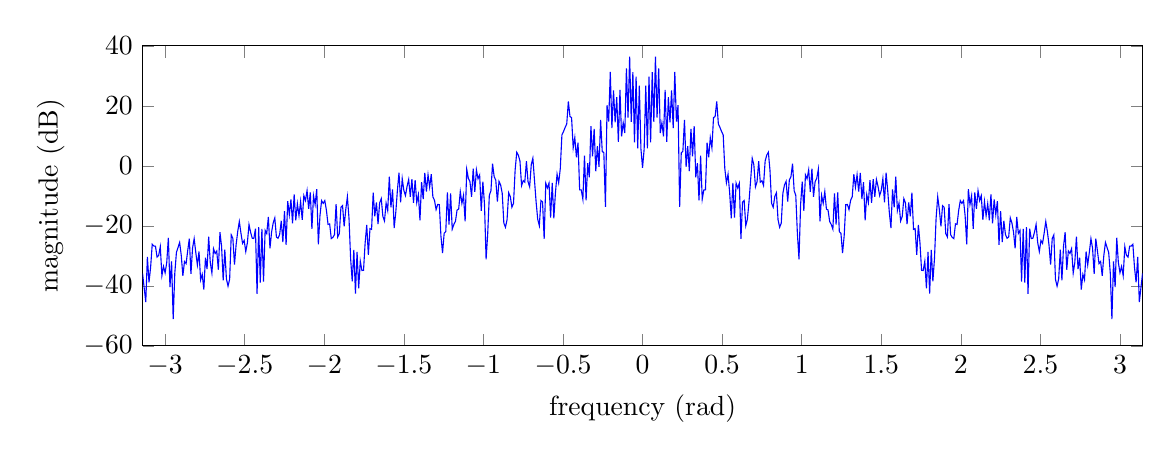
\begin{tikzpicture}

\begin{axis}[%
width=5in,
height=1.5in,
at={(1.065766in,0.414898in)},
scale only axis,
xmin=-3.14159265358979,
xmax=3.14159265358979,
xlabel={frequency (rad)},
ymin=-60,
ymax=40,
ylabel={magnitude (dB)}
]
\addplot [color=blue,solid,forget plot]
  table[row sep=crcr]{%
-3.14159265358979	-35.8436599921444\\
-3.1314584837395	-40.6397842350261\\
-3.12132431388921	-45.4114070519786\\
-3.11119014403892	-30.3657898502927\\
-3.10105597418863	-38.8408412155045\\
-3.09092180433835	-33.8558529215595\\
-3.08078763448805	-26.157133832729\\
-3.07065346463777	-26.7469609958692\\
-3.06051929478748	-26.7583668151469\\
-3.05038512493719	-30.4209416038633\\
-3.0402509550869	-29.8542153739604\\
-3.03011678523661	-26.9570278841738\\
-3.01998261538632	-36.6148164158459\\
-3.00984844553603	-33.5394392261587\\
-2.99971427568574	-35.6578649914713\\
-2.98958010583545	-32.2628942358148\\
-2.97944593598516	-23.993197586124\\
-2.96931176613487	-40.4222734901949\\
-2.95917759628458	-31.8283264690471\\
-2.94904342643429	-51.0663946579242\\
-2.938909256584	-35.7649181257139\\
-2.92877508673371	-28.8966845277701\\
-2.91864091688342	-27.2251476812973\\
-2.90850674703313	-25.5607974064893\\
-2.89837257718284	-29.8410645496576\\
-2.88823840733255	-36.6889006524956\\
-2.87810423748226	-31.9015767194902\\
-2.86797006763197	-32.601140675313\\
-2.85783589778168	-28.2676909881237\\
-2.84770172793139	-24.2820140008806\\
-2.8375675580811	-36.0527131273678\\
-2.82743338823081	-27.4498952853147\\
-2.81729921838052	-24.2998292187974\\
-2.80716504853023	-28.8668423651912\\
-2.79703087867995	-33.0484686873574\\
-2.78689670882966	-28.5832055745795\\
-2.77676253897937	-38.0157500727434\\
-2.76662836912908	-36.1885939279913\\
-2.75649419927879	-41.232199274737\\
-2.7463600294285	-30.6083701323693\\
-2.73622585957821	-34.4298621452334\\
-2.72609168972792	-23.6391506660764\\
-2.71595751987763	-32.2523249728789\\
-2.70582335002734	-35.7632689660134\\
-2.69568918017705	-27.6379325503404\\
-2.68555501032676	-29.2238816606569\\
-2.67542084047647	-28.4069669772684\\
-2.66528667062618	-34.6390153278259\\
-2.65515250077589	-22.1567848863985\\
-2.6450183309256	-26.880382005536\\
-2.63488416107531	-38.1512329753099\\
-2.62474999122502	-27.9355904342828\\
-2.61461582137473	-37.7086235875748\\
-2.60448165152444	-40.113207153787\\
-2.59434748167415	-37.8075461709975\\
-2.58421331182386	-23.0316343371797\\
-2.57407914197357	-24.2042800148477\\
-2.56394497212328	-32.9602944753443\\
-2.55381080227299	-26.3934229887756\\
-2.5436766324227	-21.9310112363369\\
-2.53354246257241	-18.5882432347269\\
-2.52340829272212	-22.4230984929961\\
-2.51327412287183	-25.8493222305387\\
-2.50313995302154	-24.9017274511297\\
-2.49300578317126	-28.5770440777079\\
-2.48287161332097	-25.6328007251073\\
-2.47273744347068	-19.5742663314655\\
-2.46260327362039	-22.1668467815201\\
-2.4524691037701	-24.1391719534506\\
-2.44233493391981	-24.2460354899214\\
-2.43220076406952	-20.975954980393\\
-2.42206659421923	-42.7079242082377\\
-2.41193242436894	-20.4794099848044\\
-2.40179825451865	-38.9666630017508\\
-2.39166408466836	-20.9983202061486\\
-2.38152991481807	-38.6296112374141\\
-2.37139574496778	-21.534230386714\\
-2.36126157511749	-22.5721445567607\\
-2.3511274052672	-17.0568568529776\\
-2.34099323541691	-27.533333035489\\
-2.33085906556662	-22.0978715782466\\
-2.32072489571633	-19.0555096095964\\
-2.31059072586604	-17.3685940697048\\
-2.30045655601575	-23.7449464757931\\
-2.29032238616546	-24.1391831460078\\
-2.28018821631517	-22.9159508044198\\
-2.27005404646488	-18.3352195505612\\
-2.25991987661459	-25.4513018685123\\
-2.2497857067643	-15.1123414237343\\
-2.23965153691401	-26.3529634682947\\
-2.22951736706372	-11.7727330320489\\
-2.21938319721343	-16.3050930379681\\
-2.20924902736314	-11.1964449090149\\
-2.19911485751286	-19.1922136578761\\
-2.18898068766257	-9.51514956144194\\
-2.17884651781228	-18.1821638325953\\
-2.16871234796199	-12.6519316511401\\
-2.1585781781117	-16.6245294192933\\
-2.14844400826141	-11.889549023497\\
-2.13830983841112	-18.0261534094626\\
-2.12817566856083	-9.96392364317686\\
-2.11804149871054	-11.5879685293564\\
-2.10790732886025	-8.29616868908074\\
-2.09777315900996	-14.3594428241051\\
-2.08763898915967	-8.8943211865756\\
-2.07750481930938	-21.0241767389362\\
-2.06737064945909	-10.0071945523245\\
-2.0572364796088	-12.9149671278638\\
-2.04710230975851	-7.80787470799636\\
-2.03696813990822	-26.1504249095737\\
-2.02683397005793	-16.6535264418017\\
-2.01669980020764	-11.6107177824673\\
-2.00656563035735	-12.5283032864379\\
-1.99643146050706	-11.6107829369912\\
-1.98629729065677	-14.8585175441363\\
-1.97616312080648	-19.5253077295878\\
-1.96602895095619	-19.3605996934909\\
-1.9558947811059	-24.2578712023889\\
-1.94576061125561	-23.8878904746756\\
-1.93562644140532	-22.9521568842458\\
-1.92549227155503	-12.7491451183413\\
-1.91535810170474	-23.7354191924265\\
-1.90522393185446	-22.6012096871204\\
-1.89508976200417	-13.8403139001484\\
-1.88495559215388	-13.2796754445027\\
-1.87482142230359	-20.1911540288229\\
-1.8646872524533	-14.5397157489642\\
-1.85455308260301	-10.3126842174127\\
-1.84441891275272	-17.483050013696\\
-1.83428474290243	-30.8698322803899\\
-1.82415057305214	-38.5421275784918\\
-1.81401640320185	-28.0371250700492\\
-1.80388223335156	-42.5928001196538\\
-1.79374806350127	-28.7386371287842\\
-1.78361389365098	-40.8899676162261\\
-1.77347972380069	-31.8014888915274\\
-1.7633455539504	-34.887463303962\\
-1.75321138410011	-34.8743536354569\\
-1.74307721424982	-25.7471151639181\\
-1.73294304439953	-19.7041051361399\\
-1.72280887454924	-29.696820716044\\
-1.71267470469895	-20.9497462951928\\
-1.70254053484866	-21.1909532558951\\
-1.69240636499837	-8.95913135483582\\
-1.68227219514808	-16.8210430321288\\
-1.67213802529779	-12.1768061099727\\
-1.6620038554475	-19.4674830825269\\
-1.65186968559721	-12.3792016035634\\
-1.64173551574692	-10.9530603502229\\
-1.63160134589663	-16.8724477022818\\
-1.62146717604634	-18.39357289372\\
-1.61133300619606	-12.439540789659\\
-1.60119883634577	-14.9056365158639\\
-1.59106466649548	-3.61870064844889\\
-1.58093049664519	-13.8689694657296\\
-1.5707963267949	-7.89431343443638\\
-1.56066215694461	-20.7447844644185\\
-1.55052798709432	-15.5475105669891\\
-1.54039381724403	-8.27217306659288\\
-1.53025964739374	-2.32647539197295\\
-1.52012547754345	-12.1683936103969\\
-1.50999130769316	-4.2754563811773\\
-1.49985713784287	-8.1944867493729\\
-1.48972296799258	-9.90763435862356\\
-1.47958879814229	-6.87433329236849\\
-1.469454628292	-4.5632349078683\\
-1.45932045844171	-10.3234549500033\\
-1.44918628859142	-4.44432906549038\\
-1.43905211874113	-12.3268173567112\\
-1.42891794889084	-4.7516963015957\\
-1.41878377904055	-12.2495481552569\\
-1.40864960919026	-9.59411872171387\\
-1.39851543933997	-18.1541821130972\\
-1.38838126948968	-5.42046890402998\\
-1.37824709963939	-11.0740688303302\\
-1.3681129297891	-2.3366185822652\\
-1.35797875993881	-8.61677161038325\\
-1.34784459008852	-2.97734557564765\\
-1.33771042023823	-7.10531019844278\\
-1.32757625038794	-2.82071557390821\\
-1.31744208053766	-10.3343416101404\\
-1.30730791068737	-11.5059666951229\\
-1.29717374083708	-14.5933403690866\\
-1.28703957098679	-12.8835217697104\\
-1.2769054011365	-12.9541019922265\\
-1.26677123128621	-23.400791898746\\
-1.25663706143592	-29.0912821166426\\
-1.24650289158563	-22.4724930332325\\
-1.23636872173534	-21.9568656613879\\
-1.22623455188505	-8.88892085576351\\
-1.21610038203476	-19.5791085249808\\
-1.20596621218447	-9.18146930404369\\
-1.19583204233418	-21.1170185806638\\
-1.18569787248389	-19.5767340699123\\
-1.1755637026336	-18.5132870888747\\
-1.16542953278331	-14.7326421099985\\
-1.15529536293302	-14.4258379832491\\
-1.14516119308273	-8.61217622542235\\
-1.13502702323244	-12.5286535118843\\
-1.12489285338215	-9.87444026012274\\
-1.11475868353186	-18.520710782111\\
-1.10462451368157	-1.16983883328066\\
-1.09449034383128	-4.16094010432891\\
-1.08435617398099	-5.29951286163618\\
-1.0742220041307	-10.3155783846455\\
-1.06408783428041	-0.913719850448168\\
-1.05395366443012	-8.70171925141733\\
-1.04381949457983	-1.34273985383032\\
-1.03368532472954	-4.31581466265128\\
-1.02355115487926	-3.04243473756471\\
-1.01341698502897	-15.021958596256\\
-1.00328281517868	-5.29568009350039\\
-0.993148645328386	-12.8089858583563\\
-0.983014475478097	-31.1500409297397\\
-0.972880305627807	-22.6030961723642\\
-0.962746135777517	-9.83003091596125\\
-0.952611965927228	-8.3211210749391\\
-0.942477796076938	0.743454973743254\\
-0.932343626226648	-3.65511337442409\\
-0.922209456376359	-4.76180760794891\\
-0.912075286526069	-11.9210121656168\\
-0.901941116675779	-5.19131165996416\\
-0.89180694682549	-6.35354184370919\\
-0.8816727769752	-9.18253710793958\\
-0.87153860712491	-19.0966634838142\\
-0.861404437274621	-20.4942778417272\\
-0.851270267424331	-17.9460663651781\\
-0.841136097574041	-8.98419759214084\\
-0.831001927723752	-10.2226358523168\\
-0.820867757873462	-13.8124654619348\\
-0.810733588023172	-12.5168981449148\\
-0.800599418172883	-1.45554022036414\\
-0.790465248322593	4.5095610902467\\
-0.780331078472303	3.55491783600218\\
-0.770196908622014	1.55995178247618\\
-0.760062738771724	-6.58030705305588\\
-0.749928568921434	-4.95813202547031\\
-0.739794399071145	-5.45862250028518\\
-0.729660229220855	1.51046230723461\\
-0.719526059370566	-5.30889767852118\\
-0.709391889520276	-7.01215393562501\\
-0.699257719669986	0.357577320852092\\
-0.689123549819697	2.51384038840824\\
-0.678989379969407	-4.80769022300247\\
-0.668855210119117	-11.9969576711807\\
-0.658721040268828	-17.8075160593182\\
-0.648586870418538	-19.9783953268986\\
-0.638452700568248	-11.5708790025062\\
-0.628318530717959	-12.0625283258628\\
-0.618184360867669	-24.3452182966423\\
-0.608050191017379	-5.8187750149795\\
-0.59791602116709	-7.38911842054282\\
-0.5877818513168	-5.75921899082423\\
-0.57764768146651	-17.258975548298\\
-0.567513511616221	-5.69562925269501\\
-0.557379341765931	-17.5004844204785\\
-0.547245171915641	-8.900830886454\\
-0.537111002065352	-2.7961103108066\\
-0.526976832215062	-5.66731575158876\\
-0.516842662364772	-0.914249761705724\\
-0.506708492514483	10.2831293117686\\
-0.496574322664193	11.4350181575122\\
-0.486440152813903	12.7847761301728\\
-0.476305982963614	13.9642998019194\\
-0.466171813113324	21.4701295585094\\
-0.456037643263035	16.4311771895226\\
-0.445903473412745	16.051502073808\\
-0.435769303562455	6.0082973830022\\
-0.425635133712166	9.39380355875547\\
-0.415500963861876	2.79810877046214\\
-0.405366794011586	7.74028035943637\\
-0.395232624161297	-8.01772111922761\\
-0.385098454311007	-8.05334276752725\\
-0.374964284460717	-11.1387670412535\\
-0.364830114610428	3.41385535476654\\
-0.354695944760138	-11.4950252028983\\
-0.344561774909848	0.878430666233941\\
-0.334427605059559	-3.81963870442518\\
-0.324293435209269	13.2228415954131\\
-0.314159265358979	3.16628532565552\\
-0.30402509550869	12.3349281760502\\
-0.2938909256584	-1.80543086969444\\
-0.28375675580811	6.57706438806299\\
-0.273622585957821	-0.341962236244982\\
-0.263488416107531	15.3056844205046\\
-0.253354246257241	4.84178812716383\\
-0.243220076406952	4.34019539837797\\
-0.233085906556662	-13.68514330626\\
-0.222951736706372	20.1929540233948\\
-0.212817566856083	14.7283865532389\\
-0.202683397005793	31.2719200858172\\
-0.192549227155503	12.5810957115038\\
-0.182415057305214	25.11706101216\\
-0.172280887454924	14.5151523815431\\
-0.162146717604634	22.8488609999694\\
-0.152012547754345	7.97498728087492\\
-0.141878377904055	25.2640717431077\\
-0.131744208053766	9.78612828550305\\
-0.121610038203476	14.3517061029633\\
-0.111475868353186	10.9470082951893\\
-0.101341698502897	32.5096623922417\\
-0.0912075286526069	16.0306960332739\\
-0.0810733588023172	36.4265083998516\\
-0.0709391889520276	14.6146749802946\\
-0.0608050191017379	31.2301043420014\\
-0.0506708492514483	7.7953345710169\\
-0.0405366794011586	29.700100910654\\
-0.030402509550869	5.79227321930543\\
-0.0202683397005793	26.7352238010944\\
-0.0101341698502897	5.61727047014028\\
0	-0.645621806738404\\
0.0101341698502897	5.61727047014028\\
0.0202683397005793	26.7352238010944\\
0.030402509550869	5.79227321930543\\
0.0405366794011586	29.700100910654\\
0.0506708492514483	7.7953345710169\\
0.0608050191017379	31.2301043420014\\
0.0709391889520276	14.6146749802946\\
0.0810733588023172	36.4265083998516\\
0.0912075286526069	16.0306960332739\\
0.101341698502897	32.5096623922417\\
0.111475868353186	10.9470082951893\\
0.121610038203476	14.3517061029633\\
0.131744208053766	9.78612828550305\\
0.141878377904055	25.2640717431077\\
0.152012547754345	7.97498728087492\\
0.162146717604634	22.8488609999694\\
0.172280887454924	14.5151523815431\\
0.182415057305214	25.11706101216\\
0.192549227155503	12.5810957115038\\
0.202683397005793	31.2719200858172\\
0.212817566856083	14.7283865532389\\
0.222951736706372	20.1929540233948\\
0.233085906556662	-13.68514330626\\
0.243220076406952	4.34019539837797\\
0.253354246257241	4.84178812716383\\
0.263488416107531	15.3056844205046\\
0.273622585957821	-0.341962236244982\\
0.28375675580811	6.57706438806299\\
0.2938909256584	-1.80543086969444\\
0.30402509550869	12.3349281760502\\
0.314159265358979	3.16628532565552\\
0.324293435209269	13.2228415954131\\
0.334427605059559	-3.81963870442518\\
0.344561774909848	0.878430666233941\\
0.354695944760138	-11.4950252028983\\
0.364830114610428	3.41385535476654\\
0.374964284460717	-11.1387670412535\\
0.385098454311007	-8.05334276752725\\
0.395232624161297	-8.01772111922761\\
0.405366794011586	7.74028035943637\\
0.415500963861876	2.79810877046214\\
0.425635133712166	9.39380355875547\\
0.435769303562455	6.0082973830022\\
0.445903473412745	16.051502073808\\
0.456037643263035	16.4311771895226\\
0.466171813113324	21.4701295585094\\
0.476305982963614	13.9642998019194\\
0.486440152813903	12.7847761301728\\
0.496574322664193	11.4350181575122\\
0.506708492514483	10.2831293117686\\
0.516842662364772	-0.914249761705724\\
0.526976832215062	-5.66731575158876\\
0.537111002065352	-2.7961103108066\\
0.547245171915641	-8.900830886454\\
0.557379341765931	-17.5004844204785\\
0.567513511616221	-5.69562925269501\\
0.57764768146651	-17.258975548298\\
0.5877818513168	-5.75921899082423\\
0.59791602116709	-7.38911842054282\\
0.608050191017379	-5.8187750149795\\
0.618184360867669	-24.3452182966423\\
0.628318530717959	-12.0625283258628\\
0.638452700568248	-11.5708790025062\\
0.648586870418538	-19.9783953268986\\
0.658721040268828	-17.8075160593182\\
0.668855210119117	-11.9969576711807\\
0.678989379969407	-4.80769022300247\\
0.689123549819697	2.51384038840824\\
0.699257719669986	0.357577320852092\\
0.709391889520276	-7.01215393562501\\
0.719526059370566	-5.30889767852118\\
0.729660229220855	1.51046230723461\\
0.739794399071145	-5.45862250028518\\
0.749928568921434	-4.95813202547031\\
0.760062738771724	-6.58030705305588\\
0.770196908622014	1.55995178247618\\
0.780331078472303	3.55491783600218\\
0.790465248322593	4.5095610902467\\
0.800599418172883	-1.45554022036414\\
0.810733588023172	-12.5168981449148\\
0.820867757873462	-13.8124654619348\\
0.831001927723752	-10.2226358523168\\
0.841136097574041	-8.98419759214084\\
0.851270267424331	-17.9460663651781\\
0.861404437274621	-20.4942778417272\\
0.87153860712491	-19.0966634838142\\
0.8816727769752	-9.18253710793958\\
0.89180694682549	-6.35354184370919\\
0.901941116675779	-5.19131165996416\\
0.912075286526069	-11.9210121656168\\
0.922209456376359	-4.76180760794891\\
0.932343626226648	-3.65511337442409\\
0.942477796076938	0.743454973743254\\
0.952611965927228	-8.3211210749391\\
0.962746135777517	-9.83003091596125\\
0.972880305627807	-22.6030961723642\\
0.983014475478097	-31.1500409297397\\
0.993148645328386	-12.8089858583563\\
1.00328281517868	-5.29568009350039\\
1.01341698502897	-15.021958596256\\
1.02355115487926	-3.04243473756471\\
1.03368532472954	-4.31581466265128\\
1.04381949457983	-1.34273985383032\\
1.05395366443012	-8.70171925141733\\
1.06408783428041	-0.913719850448168\\
1.0742220041307	-10.3155783846455\\
1.08435617398099	-5.29951286163618\\
1.09449034383128	-4.16094010432891\\
1.10462451368157	-1.16983883328066\\
1.11475868353186	-18.520710782111\\
1.12489285338215	-9.87444026012274\\
1.13502702323244	-12.5286535118843\\
1.14516119308273	-8.61217622542235\\
1.15529536293302	-14.4258379832491\\
1.16542953278331	-14.7326421099985\\
1.1755637026336	-18.5132870888747\\
1.18569787248389	-19.5767340699123\\
1.19583204233418	-21.1170185806638\\
1.20596621218447	-9.18146930404369\\
1.21610038203476	-19.5791085249808\\
1.22623455188505	-8.88892085576351\\
1.23636872173534	-21.9568656613879\\
1.24650289158563	-22.4724930332325\\
1.25663706143592	-29.0912821166426\\
1.26677123128621	-23.400791898746\\
1.2769054011365	-12.9541019922265\\
1.28703957098679	-12.8835217697104\\
1.29717374083708	-14.5933403690866\\
1.30730791068737	-11.5059666951229\\
1.31744208053766	-10.3343416101404\\
1.32757625038794	-2.82071557390821\\
1.33771042023823	-7.10531019844278\\
1.34784459008852	-2.97734557564765\\
1.35797875993881	-8.61677161038325\\
1.3681129297891	-2.3366185822652\\
1.37824709963939	-11.0740688303302\\
1.38838126948968	-5.42046890402998\\
1.39851543933997	-18.1541821130972\\
1.40864960919026	-9.59411872171387\\
1.41878377904055	-12.2495481552569\\
1.42891794889084	-4.7516963015957\\
1.43905211874113	-12.3268173567112\\
1.44918628859142	-4.44432906549038\\
1.45932045844171	-10.3234549500033\\
1.469454628292	-4.5632349078683\\
1.47958879814229	-6.87433329236849\\
1.48972296799258	-9.90763435862356\\
1.49985713784287	-8.1944867493729\\
1.50999130769316	-4.2754563811773\\
1.52012547754345	-12.1683936103969\\
1.53025964739374	-2.32647539197295\\
1.54039381724403	-8.27217306659288\\
1.55052798709432	-15.5475105669891\\
1.56066215694461	-20.7447844644185\\
1.5707963267949	-7.89431343443638\\
1.58093049664519	-13.8689694657296\\
1.59106466649548	-3.61870064844889\\
1.60119883634577	-14.9056365158639\\
1.61133300619606	-12.439540789659\\
1.62146717604634	-18.39357289372\\
1.63160134589663	-16.8724477022818\\
1.64173551574692	-10.9530603502229\\
1.65186968559721	-12.3792016035634\\
1.6620038554475	-19.4674830825269\\
1.67213802529779	-12.1768061099727\\
1.68227219514808	-16.8210430321288\\
1.69240636499837	-8.95913135483582\\
1.70254053484866	-21.1909532558951\\
1.71267470469895	-20.9497462951928\\
1.72280887454924	-29.696820716044\\
1.73294304439953	-19.7041051361399\\
1.74307721424982	-25.7471151639181\\
1.75321138410011	-34.8743536354569\\
1.7633455539504	-34.887463303962\\
1.77347972380069	-31.8014888915274\\
1.78361389365098	-40.8899676162261\\
1.79374806350127	-28.7386371287842\\
1.80388223335156	-42.5928001196538\\
1.81401640320185	-28.0371250700492\\
1.82415057305214	-38.5421275784918\\
1.83428474290243	-30.8698322803899\\
1.84441891275272	-17.483050013696\\
1.85455308260301	-10.3126842174127\\
1.8646872524533	-14.5397157489642\\
1.87482142230359	-20.1911540288229\\
1.88495559215388	-13.2796754445027\\
1.89508976200417	-13.8403139001484\\
1.90522393185446	-22.6012096871204\\
1.91535810170474	-23.7354191924265\\
1.92549227155503	-12.7491451183413\\
1.93562644140532	-22.9521568842458\\
1.94576061125561	-23.8878904746756\\
1.9558947811059	-24.2578712023889\\
1.96602895095619	-19.3605996934909\\
1.97616312080648	-19.5253077295878\\
1.98629729065677	-14.8585175441363\\
1.99643146050706	-11.6107829369912\\
2.00656563035735	-12.5283032864379\\
2.01669980020764	-11.6107177824673\\
2.02683397005793	-16.6535264418017\\
2.03696813990822	-26.1504249095737\\
2.04710230975851	-7.80787470799636\\
2.0572364796088	-12.9149671278638\\
2.06737064945909	-10.0071945523245\\
2.07750481930938	-21.0241767389362\\
2.08763898915967	-8.8943211865756\\
2.09777315900996	-14.3594428241051\\
2.10790732886025	-8.29616868908074\\
2.11804149871054	-11.5879685293564\\
2.12817566856083	-9.96392364317686\\
2.13830983841112	-18.0261534094626\\
2.14844400826141	-11.889549023497\\
2.1585781781117	-16.6245294192933\\
2.16871234796199	-12.6519316511401\\
2.17884651781228	-18.1821638325953\\
2.18898068766257	-9.51514956144194\\
2.19911485751286	-19.1922136578761\\
2.20924902736314	-11.1964449090149\\
2.21938319721343	-16.3050930379681\\
2.22951736706372	-11.7727330320489\\
2.23965153691401	-26.3529634682947\\
2.2497857067643	-15.1123414237343\\
2.25991987661459	-25.4513018685123\\
2.27005404646488	-18.3352195505612\\
2.28018821631517	-22.9159508044198\\
2.29032238616546	-24.1391831460078\\
2.30045655601575	-23.7449464757931\\
2.31059072586604	-17.3685940697048\\
2.32072489571633	-19.0555096095964\\
2.33085906556662	-22.0978715782466\\
2.34099323541691	-27.533333035489\\
2.3511274052672	-17.0568568529776\\
2.36126157511749	-22.5721445567607\\
2.37139574496778	-21.534230386714\\
2.38152991481807	-38.6296112374141\\
2.39166408466836	-20.9983202061486\\
2.40179825451865	-38.9666630017508\\
2.41193242436894	-20.4794099848044\\
2.42206659421923	-42.7079242082377\\
2.43220076406952	-20.975954980393\\
2.44233493391981	-24.2460354899214\\
2.4524691037701	-24.1391719534506\\
2.46260327362039	-22.1668467815201\\
2.47273744347068	-19.5742663314655\\
2.48287161332097	-25.6328007251073\\
2.49300578317126	-28.5770440777079\\
2.50313995302154	-24.9017274511297\\
2.51327412287183	-25.8493222305387\\
2.52340829272212	-22.4230984929961\\
2.53354246257241	-18.5882432347269\\
2.5436766324227	-21.9310112363369\\
2.55381080227299	-26.3934229887756\\
2.56394497212328	-32.9602944753443\\
2.57407914197357	-24.2042800148477\\
2.58421331182386	-23.0316343371797\\
2.59434748167415	-37.8075461709975\\
2.60448165152444	-40.113207153787\\
2.61461582137473	-37.7086235875748\\
2.62474999122502	-27.9355904342828\\
2.63488416107531	-38.1512329753099\\
2.6450183309256	-26.880382005536\\
2.65515250077589	-22.1567848863985\\
2.66528667062618	-34.6390153278259\\
2.67542084047647	-28.4069669772684\\
2.68555501032676	-29.2238816606569\\
2.69568918017705	-27.6379325503404\\
2.70582335002734	-35.7632689660134\\
2.71595751987763	-32.2523249728789\\
2.72609168972792	-23.6391506660764\\
2.73622585957821	-34.4298621452334\\
2.7463600294285	-30.6083701323693\\
2.75649419927879	-41.232199274737\\
2.76662836912908	-36.1885939279913\\
2.77676253897937	-38.0157500727434\\
2.78689670882966	-28.5832055745795\\
2.79703087867995	-33.0484686873574\\
2.80716504853023	-28.8668423651912\\
2.81729921838052	-24.2998292187974\\
2.82743338823081	-27.4498952853147\\
2.8375675580811	-36.0527131273678\\
2.84770172793139	-24.2820140008806\\
2.85783589778168	-28.2676909881237\\
2.86797006763197	-32.601140675313\\
2.87810423748226	-31.9015767194902\\
2.88823840733255	-36.6889006524956\\
2.89837257718284	-29.8410645496576\\
2.90850674703313	-25.5607974064893\\
2.91864091688342	-27.2251476812973\\
2.92877508673371	-28.8966845277701\\
2.938909256584	-35.7649181257139\\
2.94904342643429	-51.0663946579242\\
2.95917759628458	-31.8283264690471\\
2.96931176613487	-40.4222734901949\\
2.97944593598516	-23.993197586124\\
2.98958010583545	-32.2628942358148\\
2.99971427568574	-35.6578649914713\\
3.00984844553603	-33.5394392261587\\
3.01998261538632	-36.6148164158459\\
3.03011678523661	-26.9570278841738\\
3.0402509550869	-29.8542153739604\\
3.05038512493719	-30.4209416038633\\
3.06051929478748	-26.7583668151469\\
3.07065346463777	-26.7469609958692\\
3.08078763448805	-26.157133832729\\
3.09092180433835	-33.8558529215595\\
3.10105597418863	-38.8408412155045\\
3.11119014403892	-30.3657898502927\\
3.12132431388921	-45.4114070519786\\
3.1314584837395	-40.6397842350261\\
3.14159265358979	-35.8436599921444\\
};
\end{axis}
\end{tikzpicture}%

\caption{DFT of the windowed speech signal}
\label{fig:dftsig}
\end{figure}

\begin{figure}[H]
\centering
% This file was created by matlab2tikz.
% Minimal pgfplots version: 1.3
%
%The latest updates can be retrieved from
%  http://www.mathworks.com/matlabcentral/fileexchange/22022-matlab2tikz
%where you can also make suggestions and rate matlab2tikz.
%
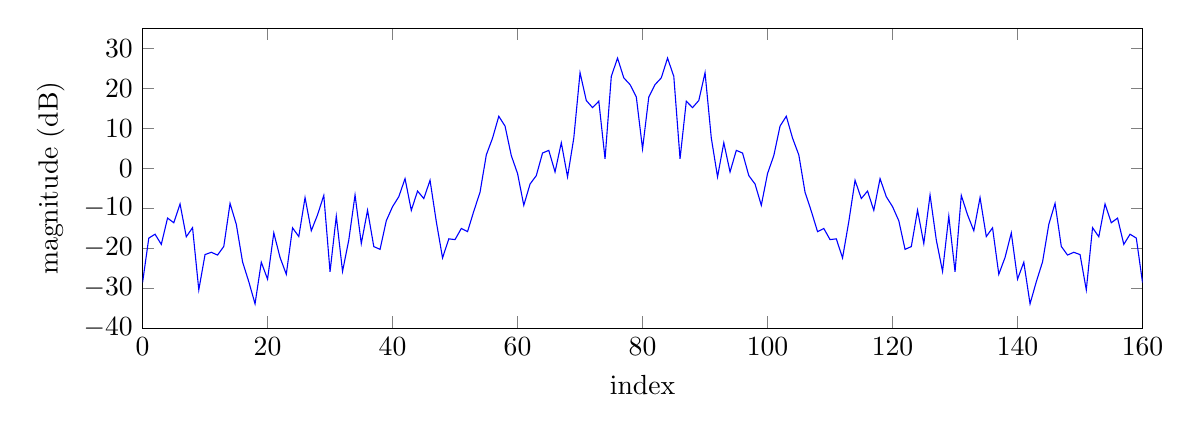
\begin{tikzpicture}

\begin{axis}[%
width=5in,
height=1.5in,
at={(1.065766in,0.414898in)},
scale only axis,
xmin=0,
xmax=160,
xlabel={index},
ymin=-40,
ymax=35,
ytick={-40, -30, -20, -10,   0,  10,  20,  30},
ylabel={magnitude (dB)}
]
\addplot [color=blue,solid,forget plot]
  table[row sep=crcr]{%
0	-28.6125162916474\\
1	-17.4704733387227\\
2	-16.5016761797241\\
3	-19.037630311822\\
4	-12.4709939875443\\
5	-13.6362092226996\\
6	-8.92724520000263\\
7	-17.1378067858692\\
8	-14.8648478263642\\
9	-30.4099984476106\\
10	-21.5910051816587\\
11	-21.0198678704044\\
12	-21.7118567048747\\
13	-19.5513286472656\\
14	-8.79054594700713\\
15	-14.0326071209007\\
16	-23.4099782044045\\
17	-28.384232105041\\
18	-33.8981235027975\\
19	-23.5056088200162\\
20	-27.7327012696947\\
21	-16.1665505734994\\
22	-22.3091091498673\\
23	-26.5154953905981\\
24	-14.9058851678196\\
25	-17.0830291712134\\
26	-7.34651157175709\\
27	-15.6311909765472\\
28	-11.6593229524729\\
29	-6.80037084846944\\
30	-25.8834024947994\\
31	-11.9937823906139\\
32	-25.7945889334185\\
33	-17.9307374015713\\
34	-6.70599652647731\\
35	-18.8365869510729\\
36	-10.5103242416768\\
37	-19.5950848565096\\
38	-20.2833857478478\\
39	-13.1342600420935\\
40	-9.61164346993855\\
41	-7.12392120028633\\
42	-2.60196228296663\\
43	-10.5367110384536\\
44	-5.7148928518398\\
45	-7.58327099141023\\
46	-3.02200773491511\\
47	-13.3509645710631\\
48	-22.4279487970861\\
49	-17.6570657852639\\
50	-17.8509290982908\\
51	-15.0638287907441\\
52	-15.8546224171618\\
53	-10.7413511897391\\
54	-6.00166627385159\\
55	3.32952098898371\\
56	7.52677556151476\\
57	12.9880502519307\\
58	10.5341104874498\\
59	3.15696693990577\\
60	-1.32461112304062\\
61	-9.26207166086977\\
62	-3.95824701029244\\
63	-1.84664335902698\\
64	3.79952981360764\\
65	4.46059297904441\\
66	-0.931529340430169\\
67	6.36687339922219\\
68	-2.16282680814858\\
69	7.55472381180202\\
70	23.8777790904062\\
71	16.9306700123778\\
72	15.1488308078606\\
73	16.7513207692407\\
74	2.36170680457602\\
75	22.9631684355847\\
76	27.5289181077213\\
77	22.5887285499779\\
78	20.9034408569324\\
79	17.827183077013\\
80	4.84466305455452\\
81	17.827183077013\\
82	20.9034408569324\\
83	22.5887285499779\\
84	27.5289181077213\\
85	22.9631684355847\\
86	2.36170680457602\\
87	16.7513207692407\\
88	15.1488308078606\\
89	16.9306700123778\\
90	23.8777790904062\\
91	7.55472381180201\\
92	-2.1628268081486\\
93	6.36687339922219\\
94	-0.931529340430176\\
95	4.46059297904441\\
96	3.79952981360762\\
97	-1.84664335902696\\
98	-3.95824701029245\\
99	-9.26207166086975\\
100	-1.32461112304064\\
101	3.15696693990577\\
102	10.5341104874498\\
103	12.9880502519307\\
104	7.52677556151476\\
105	3.32952098898369\\
106	-6.00166627385153\\
107	-10.7413511897391\\
108	-15.8546224171618\\
109	-15.0638287907441\\
110	-17.8509290982907\\
111	-17.657065785264\\
112	-22.427948797086\\
113	-13.3509645710631\\
114	-3.02200773491512\\
115	-7.58327099141021\\
116	-5.71489285183981\\
117	-10.5367110384537\\
118	-2.60196228296661\\
119	-7.12392120028639\\
120	-9.6116434699386\\
121	-13.1342600420934\\
122	-20.2833857478478\\
123	-19.5950848565095\\
124	-10.5103242416766\\
125	-18.8365869510728\\
126	-6.70599652647736\\
127	-17.9307374015712\\
128	-25.7945889334185\\
129	-11.9937823906139\\
130	-25.8834024947989\\
131	-6.80037084846945\\
132	-11.6593229524729\\
133	-15.6311909765471\\
134	-7.3465115717571\\
135	-17.0830291712133\\
136	-14.9058851678195\\
137	-26.5154953905981\\
138	-22.3091091498673\\
139	-16.1665505734992\\
140	-27.7327012696949\\
141	-23.5056088200162\\
142	-33.8981235027973\\
143	-28.384232105041\\
144	-23.4099782044048\\
145	-14.0326071209006\\
146	-8.79054594700706\\
147	-19.5513286472662\\
148	-21.7118567048747\\
149	-21.0198678704044\\
150	-21.5910051816588\\
151	-30.40999844761\\
152	-14.8648478263642\\
153	-17.1378067858693\\
154	-8.92724520000262\\
155	-13.6362092226996\\
156	-12.4709939875443\\
157	-19.0376303118222\\
158	-16.5016761797241\\
159	-17.4704733387226\\
160	-28.6125162916474\\
};
\end{axis}
\end{tikzpicture}%

\caption{resampled DFT of the windowed speech signal}
\label{fig:resampdftsig}
\end{figure}

Finally, solving the linear system (\ref{linsys}) we get the amplitude and phase of each harmonic as shown in figure \ref{fig:harest}.

\begin{figure}[H]
\centering
% This file was created by matlab2tikz.
% Minimal pgfplots version: 1.3
%
%The latest updates can be retrieved from
%  http://www.mathworks.com/matlabcentral/fileexchange/22022-matlab2tikz
%where you can also make suggestions and rate matlab2tikz.
%
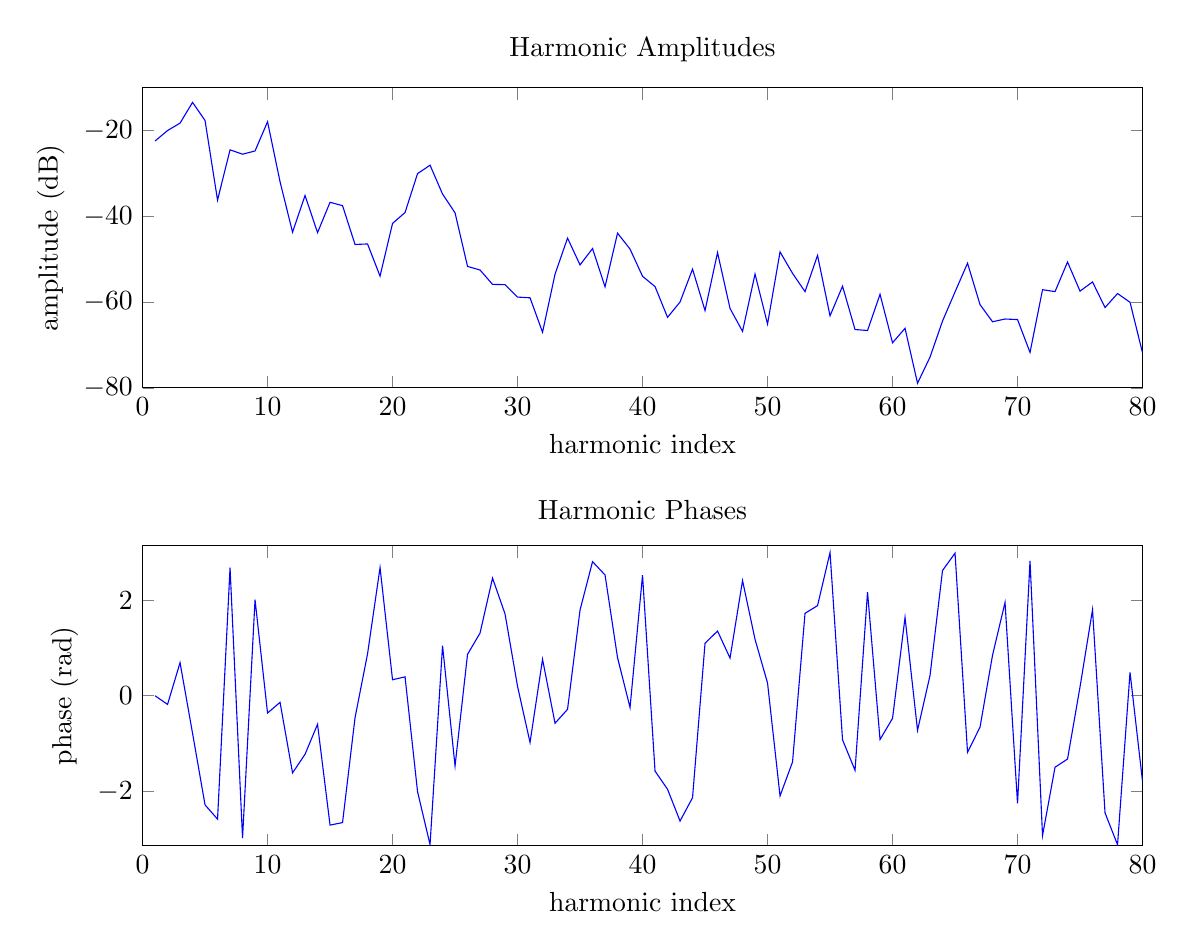
\begin{tikzpicture}

\begin{axis}[%
width=5in,
height=1.5in,
at={(1.065766in,0.510578in)},
scale only axis,
xmin=0,
xmax=80,
xlabel={harmonic index},
ymin=-3.14159265358979,
ymax=3.14159265358979,
ylabel={phase (rad)},
title={Harmonic Phases}
]
\addplot [color=blue,solid,forget plot]
  table[row sep=crcr]{%
1	0\\
2	-0.180565479753255\\
3	0.692785736966256\\
4	-0.785809306178496\\
5	-2.28586882614462\\
6	-2.58418390350478\\
7	2.68171285755527\\
8	-2.97915641537207\\
9	2.01129098404838\\
10	-0.361452873660596\\
11	-0.13778313217739\\
12	-1.61572957024156\\
13	-1.22612584687168\\
14	-0.597711932524213\\
15	-2.70907395702202\\
16	-2.65601905304139\\
17	-0.458633511801352\\
18	0.876804257779405\\
19	2.68334441770604\\
20	0.335446500045848\\
21	0.395706931238728\\
22	-2.00717826038434\\
23	-3.1175249630569\\
24	1.04977534902569\\
25	-1.46932193667427\\
26	0.867723506775725\\
27	1.31282506241202\\
28	2.46398807076242\\
29	1.71374351847756\\
30	0.197033823848784\\
31	-0.97815698112553\\
32	0.763711619453339\\
33	-0.576145756536846\\
34	-0.284243955549343\\
35	1.79605761680995\\
36	2.80883570984693\\
37	2.52948260712062\\
38	0.79712212028597\\
39	-0.245815562469559\\
40	2.52457433890326\\
41	-1.577800024915\\
42	-1.95840338387922\\
43	-2.6234081674875\\
44	-2.13538965040648\\
45	1.10004881969634\\
46	1.35499188309688\\
47	0.789524445620138\\
48	2.41178168720588\\
49	1.18182171551177\\
50	0.267232620783915\\
51	-2.0977370936475\\
52	-1.38697572225217\\
53	1.72640769346899\\
54	1.88747931305788\\
55	2.99998808157351\\
56	-0.923156857611794\\
57	-1.56174424438561\\
58	2.17021547827883\\
59	-0.916322747110598\\
60	-0.474089811269806\\
61	1.64082750515297\\
62	-0.724114712100224\\
63	0.426220993047004\\
64	2.62322379327817\\
65	2.98678441838801\\
66	-1.18472681779014\\
67	-0.656652156243645\\
68	0.848267436341409\\
69	1.95437485535922\\
70	-2.25569878566395\\
71	2.82200419174768\\
72	-2.92744412569887\\
73	-1.49646389904832\\
74	-1.32580246505923\\
75	0.18645692938405\\
76	1.80276224021446\\
77	-2.45309171949805\\
78	-3.12046334502378\\
79	0.490485242698611\\
80	-1.79357361863156\\
};
\end{axis}

\begin{axis}[%
width=5in,
height=1.5in,
at={(1.065766in,2.8in)},
scale only axis,
xmin=0,
xmax=80,
xlabel={harmonic index},
ymin=-80,
ymax=-10,
ylabel={amplitude (dB)},
title={Harmonic Amplitudes}
]
\addplot [color=blue,solid,forget plot]
  table[row sep=crcr]{%
1	-22.3990504995125\\
2	-19.9561610970265\\
3	-18.220399194944\\
4	-13.3836404464587\\
5	-17.6105776187714\\
6	-36.1895868819022\\
7	-24.4611807433244\\
8	-25.4748766103505\\
9	-24.722419471058\\
10	-17.9010069246374\\
11	-31.8889032929437\\
12	-43.666918574083\\
13	-35.1125107600728\\
14	-43.771220477003\\
15	-36.6966461413483\\
16	-37.4817575494135\\
17	-46.5420914769673\\
18	-46.4173857506402\\
19	-53.9210161514661\\
20	-41.6309515466904\\
21	-39.0869651464501\\
22	-30.0064034412142\\
23	-28.0422359492733\\
24	-34.7607286080438\\
25	-39.1559872000186\\
26	-51.6586703619142\\
27	-52.4965996174131\\
28	-55.8556574648022\\
29	-55.9104006652982\\
30	-58.8146987714252\\
31	-58.9851802019769\\
32	-67.0196726676147\\
33	-53.4674130228362\\
34	-45.0582638564354\\
35	-51.3036535612929\\
36	-47.4962869798055\\
37	-56.415494011159\\
38	-43.8941555787115\\
39	-47.6128970285629\\
40	-53.9652294957197\\
41	-56.3625274094788\\
42	-63.5413604369321\\
43	-59.9661286186982\\
44	-52.2929515072242\\
45	-61.9594129451416\\
46	-48.4291817100444\\
47	-61.4652871445808\\
48	-66.816867297986\\
49	-53.4274533629236\\
50	-65.1175914194155\\
51	-48.2730397553572\\
52	-53.2762752300459\\
53	-57.5438128527049\\
54	-49.0921963594241\\
55	-63.1899594321326\\
56	-56.2713149245891\\
57	-66.3870813671189\\
58	-66.6166982241167\\
59	-58.1655656306794\\
60	-69.4781730460634\\
61	-66.1059298179488\\
62	-78.9154384702552\\
63	-72.8138593806813\\
64	-64.4033738531943\\
65	-57.6122006038775\\
66	-50.907684094413\\
67	-60.5769286367728\\
68	-64.574264822378\\
69	-63.9331774937841\\
70	-64.0616502890338\\
71	-71.7317889810879\\
72	-57.0919428484573\\
73	-57.5410480470678\\
74	-50.6303381640701\\
75	-57.4233725659845\\
76	-55.2836514531129\\
77	-61.2593200341622\\
78	-57.9847635834788\\
79	-60.0271134266644\\
80	-71.8307000976325\\
};
\end{axis}
\end{tikzpicture}%

\caption{estimated parameters of harmonics}
\label{fig:harest}
\end{figure}

\newpage
\begin{thebibliography}{99}

%\setlength{\parskip}{-0.01cm}
\bibitem{stylianou-1996}{Stylianou, Yannis. ``Harmonic plus noise models for speech, combined with statistical methods, for speech and speaker modification." Diss. Ecole Nationale Supérieure des Télécommunications, 1996.}

\bibitem{syrdal-1998}{Syrdal, Ann, et al. ``TD-PSOLA versus harmonic plus noise model in diphone based speech synthesis." Acoustics, Speech and Signal Processing, 1998. Proceedings of the 1998 IEEE International Conference on. Vol. 1. IEEE, 1998.}

\bibitem{greengard-2004}{Greengard, Leslie, and June-Yub Lee. ``Accelerating the nonuniform fast Fourier transform." SIAM review 46.3 (2004): 443-454.}

\bibitem{smith}{Smith, Julius O. ``Spectral Audio Signal Processing." W3K Publishing. ISBN 978-0-9745607-3-1.}

\bibitem{cooley-1965}{Cooley, James W., and John W. Tukey. ``An algorithm for the machine calculation of complex Fourier series." Mathematics of computation 19.90 (1965): 297-301.}

\bibitem{george-1997}{George, E. Bryan, and Mark JT Smith. ``Speech analysis/synthesis and modification using an analysis-by-synthesis/overlap-add sinusoidal model." Speech and Audio Processing, IEEE Transactions on 5.5 (1997): 389-406.}

\bibitem{serra-1990}{Serra, Xavier, and Julius O. Smith. ``Spectral modeling synthesis: A sound analysis/synthesis system based on a deterministic plus stochastic decomposition." Computer Music Journal (1990): 12-24.}

\bibitem{hua-2014}{Hua, Kanru. ``A method to improve the extraction quality of periodic component of speech". Patent Application. CN201410457379. 2014.}

\end{thebibliography}

\end{document}
